\expandafter\newcommand\csname Slidep01\endcsname{%
\renewcommand{\defenseblock}{Introducción}
\renewcommand{\defensenav}{Defensa del TFG}
\begin{frame}[plain]\hypertarget{p01}{}
\centering
\vspace*{5mm}

\includegraphics[height=33mm]{assets/logo_uniovi_portada.pdf}\par
\vspace{6mm}
{\fontsize{32}{40}\selectfont\ThesisTitle\par}
\vspace{7mm}
{\fontsize{19}{25}\selectfont\DegreeName\par}
\vspace{6mm}
{\fontsize{21}{27}\selectfont\AuthorName\par}
{\fontsize{17}{23}\selectfont Tutor: \SupervisorName\par}
\vfill

\includegraphics[height=9mm]{assets/logo_epi_horizontal.pdf}\hfill
{\fontsize{17}{22}\selectfont\SubmissionDate}\par
\note{Buenos días. Este TFG estudia la clasificación de imágenes de ECG con pocos ejemplos etiquetados y utiliza el síndrome de Brugada como caso de estudio.}
\end{frame}}

\expandafter\newcommand\csname Slideproblema\endcsname{%
\renewcommand{\defenseblock}{Introducción}
\renewcommand{\defensenav}{Defensa del TFG}
\begin{frame}[c]\hypertarget{problema}{}
\frametitle{Enfermedades cardiovasculares y síndrome de Brugada}
\begin{columns}[c,onlytextwidth]
\begin{column}{.56\textwidth}
\centering
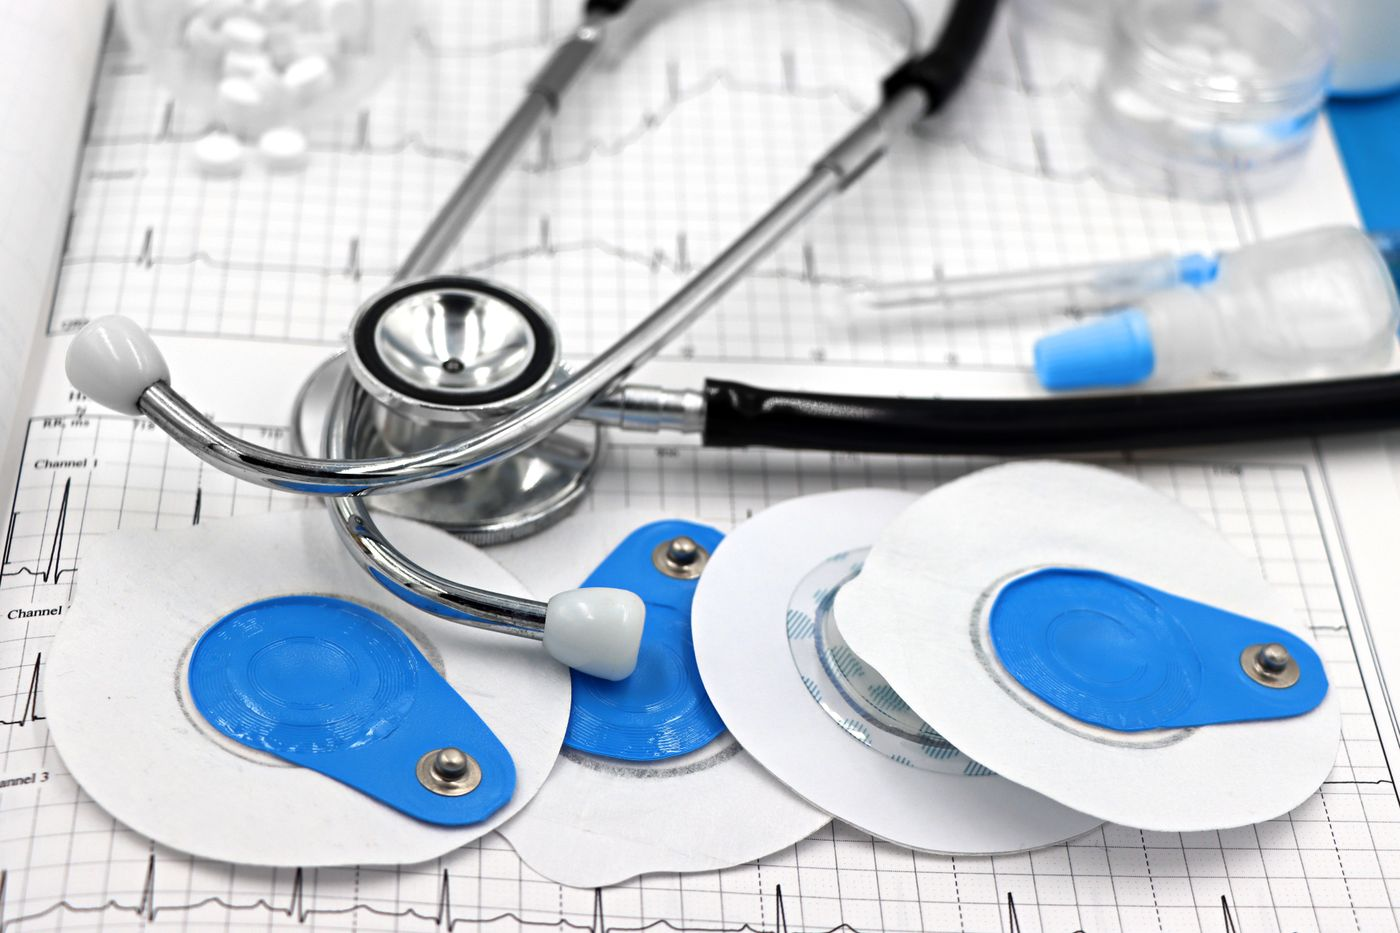
\includegraphics[width=\linewidth,height=103mm,keepaspectratio]{assets/referencias_visuales/electrodos.jpg}\par
\figurecaption{1}{\href{https://www.pexels.com/photo/medical-instruments-on-electrocardiogram-printout-35044386/}{Electrodos sobre un ECG. Marta Branco, Pexels.}}
\end{column}
\begin{column}{.39\textwidth}
{\color{UOGreen}\fontsize{42}{49}\selectfont 19,8 millones\par}
\vspace{2mm}
{\fontsize{19}{25}\selectfont de muertes cardiovasculares\\en el mundo en 2022.\par}
\credit{\href{https://www.who.int/en/news-room/fact-sheets/detail/cardiovascular-diseases-(cvds)}{Estimación de la OMS.}}
\vspace{8mm}
{\color{UOGreen}\fontsize{23}{30}\selectfont Síndrome de Brugada\par}
{\fontsize{19}{25}\selectfont Pocos positivos para\\entrenar y evaluar.\par}
\end{column}
\end{columns}
\note{La OMS estima que en 2022 murieron 19,8 millones de personas por enfermedades cardiovasculares. Dentro de ese contexto, Brugada plantea una dificultad distinta: al haber pocos casos, cuesta reunir ECG positivos confirmados que cubran la variedad de trazados y reservar suficientes positivos para evaluar el modelo. En Brugada esto importa especialmente porque el patrón puede ser intermitente, incluso en un mismo paciente.}
\end{frame}}

\expandafter\newcommand\csname Slidep02\endcsname{%
\renewcommand{\defenseblock}{Introducción}
\renewcommand{\defensenav}{Defensa del TFG}
\begin{frame}[plain]\hypertarget{p02}{}
\begin{tikzpicture}[remember picture,overlay,x=1mm,y=-1mm]
\begin{scope}[shift={(current page.north west)}]
\node[anchor=north west,inner sep=0pt] at (0,0)
  {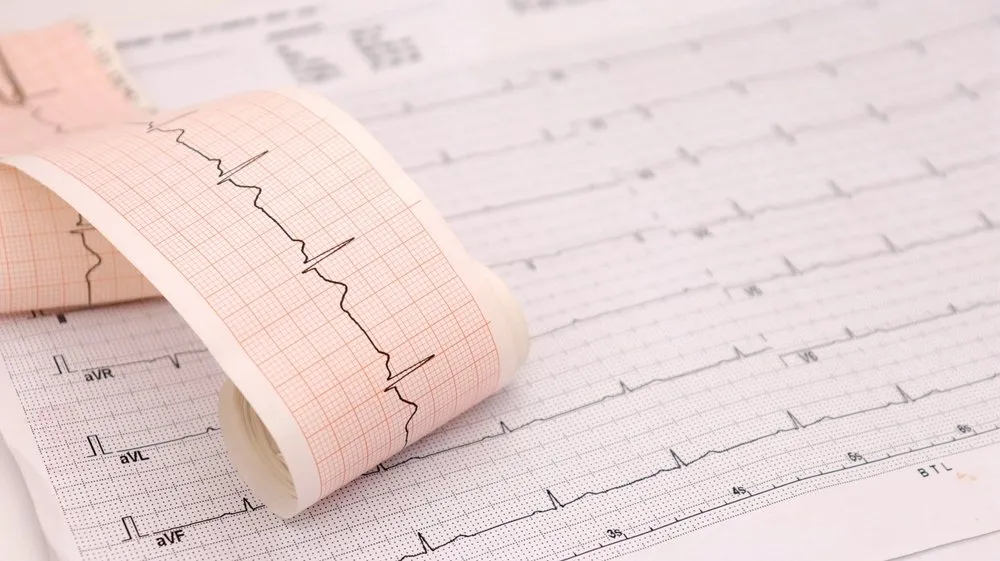
\includegraphics[viewport=0 86 1000 420,clip,width=\paperwidth]{assets/referencias_visuales/electrocardiograma_papel_adjunto.png}};
\node[anchor=north west,inner sep=0pt,text width=288mm] at (16,169)
  {\figurecaption{2}{Electrocardiograma en papel.}};
\node[anchor=north west,inner sep=0pt,text=UOInk] at (16,118)
  {\fontsize{40}{47}\selectfont Electrocardiograma en formato imagen};
\node[anchor=north west,inner sep=0pt,text=UOGreen] at (16,143)
  {\fontsize{21}{28}\selectfont ¿Puede un modelo interpretar el trazado con pocos ejemplos?};
\node[anchor=south east,inner sep=0pt,text=UOGray] at (302,172)
  {\fontsize{11}{14}\selectfont\insertframenumber};
\end{scope}
\end{tikzpicture}
\note{El análisis automático suele empezar por la señal digital, que permite medir amplitudes e intervalos. Aquí represento la señal como imagen para comprobar si un modelo de visión y lenguaje puede reconocer diferencias en la forma del trazado cuando solo tiene unos pocos ejemplos. La foto ilustra cómo se ve un ECG en papel. En el experimento, ambos modelos reciben imágenes renderizadas de un latido de V1.}
\end{frame}}

\expandafter\newcommand\csname Slidea03\endcsname{%
\renewcommand{\defenseblock}{Introducción}
\renewcommand{\defensenav}{Defensa del TFG}
\begin{frame}[c]\hypertarget{a03}{}
\frametitle{Aprendizaje en contexto}
\fullfigure[94mm]{icl_general_dong2024.pdf}
\takeaway{Instrucciones y ejemplos etiquetados orientan la respuesta a una consulta nueva, sin actualizar los pesos.}
\figurecaption{3}{Esquema de ICL en una tarea de texto, adaptado de Dong y colaboradores (2024).}
\note{A Gemma le mostramos instrucciones, varias imágenes con sus etiquetas y, al final, el ECG que queremos clasificar. Sus pesos permanecen fijos. El esquema ilustra el mismo principio con texto. En nuestro caso, cada demostración incluye un ECG y su etiqueta.}
\end{frame}}

\expandafter\newcommand\csname Slideobjetivos\endcsname{%
\renewcommand{\defenseblock}{Introducción}
\renewcommand{\defensenav}{Defensa del TFG}
\begin{frame}[c]\hypertarget{objetivos}{}
\frametitle{Propuesta y objetivos del TFG}
{\fontsize{20}{27}\selectfont\color{UOGreen} Apoyar el triaje de ECG sospechosos.\par}
\vspace{8mm}
{\fontsize{25}{34}\selectfont
{\color{UOGreen}01}\quad Efecto del número de demostraciones\par\vspace{10mm}
{\color{UOGreen}02}\quad Comparación del ICL con una CNN supervisada\par\vspace{10mm}
{\color{UOGreen}03}\quad Transferencia de datos sintéticos a datos clínicos\par}
\note{La pregunta principal es si Gemma 4 puede aprovechar pocos ECG etiquetados para clasificar un trazado nuevo. Primero estudio el efecto del número de demostraciones. Después comparo el ICL con ResNet18, que emplea los casos para entrenar. La tercera pregunta es cuánto se conserva al pasar de ejemplos sintéticos a ECG clínicos.}
\end{frame}}

\expandafter\newcommand\csname Slideindice\endcsname{%
\renewcommand{\defenseblock}{Introducción}
\renewcommand{\defensenav}{Defensa del TFG}
\begin{frame}[c]\hypertarget{indice}{}
\frametitle{Estructura de la exposición}
{\fontsize{25}{34}\selectfont
\hyperlink{antecedentes}{1. Estado del arte y fundamentos}\par\vspace{7mm}
\hyperlink{p05}{2. Datos, simulación e implementación}\par\vspace{7mm}
\hyperlink{escenarios}{3. Escenarios y protocolo de evaluación}\par\vspace{7mm}
\hyperlink{escenario_simulador}{4. Resultados en los tres escenarios}\par\vspace{7mm}
\hyperlink{p16}{5. Conclusiones, discusión y continuación}\par}
\note{Primero sitúo la propuesta en el estado del arte y presento el caso de Brugada. Después explico los datos, el diseño y el protocolo. Los resultados siguen los tres escenarios de evaluación.}
\end{frame}}

\expandafter\newcommand\csname Slideantecedentes\endcsname{%
\renewcommand{\defenseblock}{Introducción}
\renewcommand{\defensenav}{Defensa del TFG}
\begin{frame}[c]\hypertarget{antecedentes}{}
\frametitle{Estado del arte}
\begin{columns}[c,onlytextwidth]
\begin{column}{.49\textwidth}
\centering
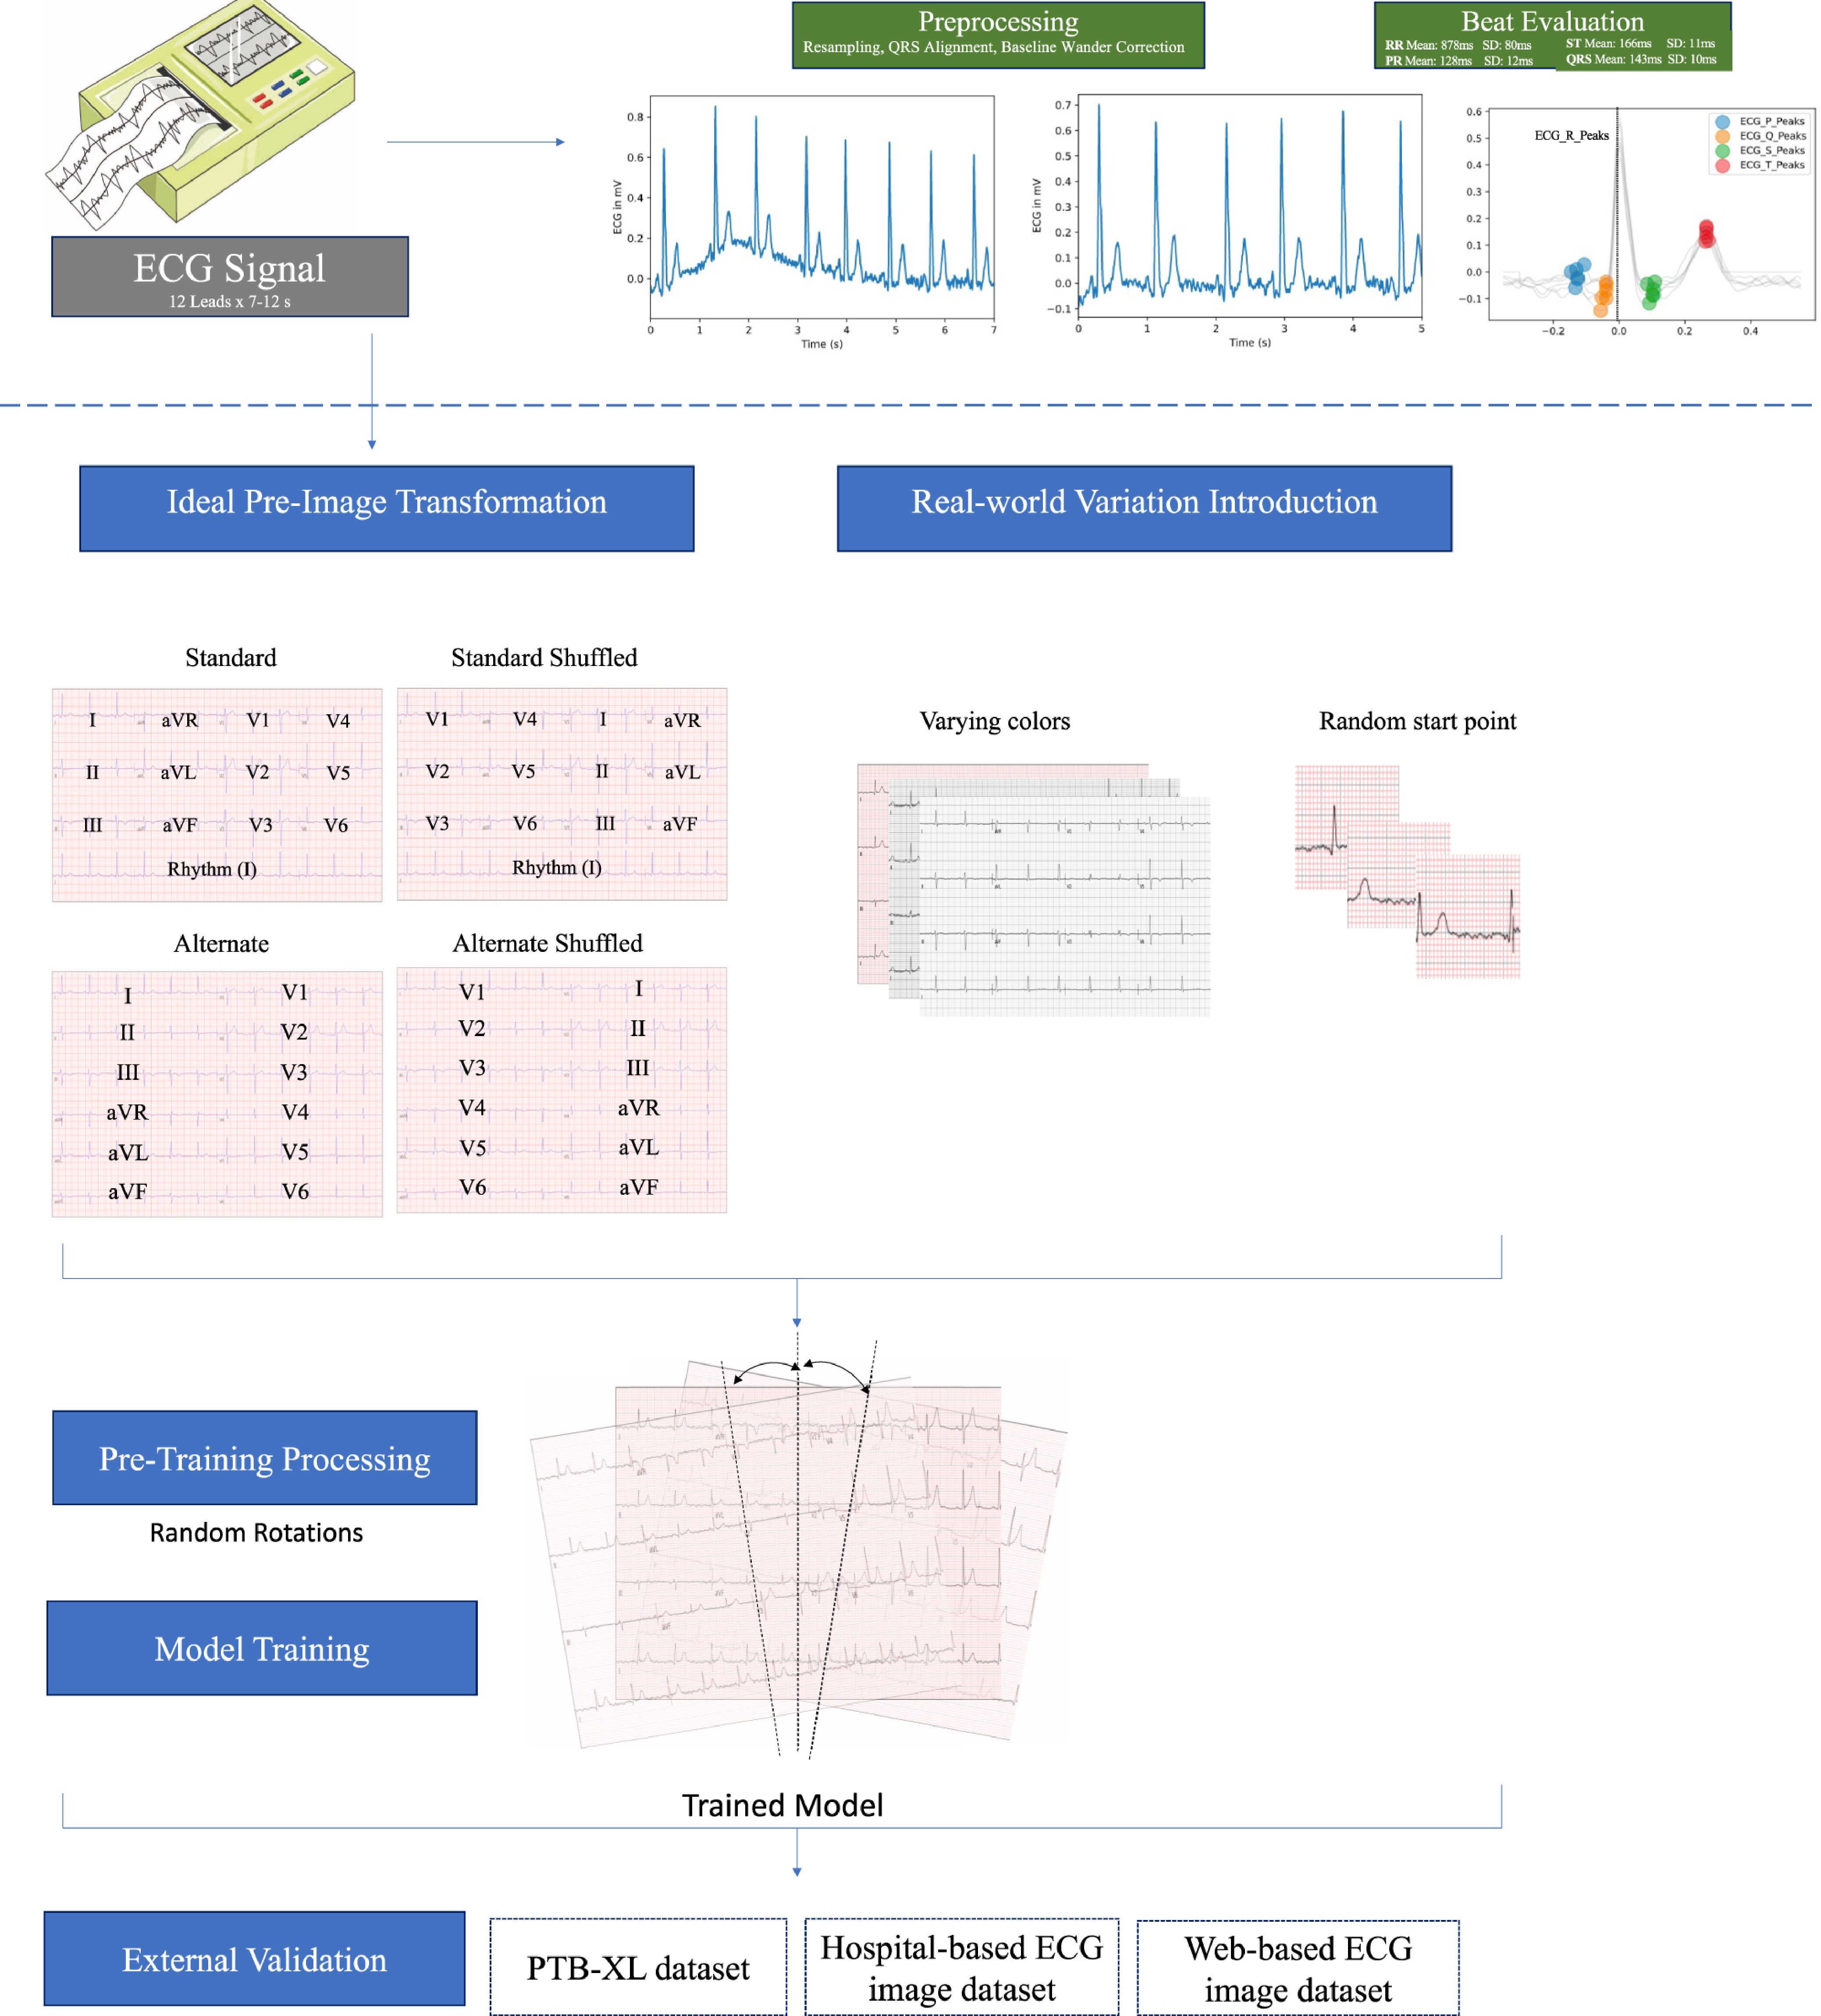
\includegraphics[trim=0 735bp 0 0,clip,width=\linewidth,height=95mm,keepaspectratio]{assets/referencias_visuales/sangha.pdf}\par
\figurecaption{4}{Conversión de señal a imagen. Sangha et al. (2022), CC BY 4.0.}
\end{column}
\begin{column}{.46\textwidth}
{\color{UOGreen}\fontsize{24}{30}\selectfont ECG como señal\par}
{\fontsize{19}{26}\selectfont Ribeiro et al. (2020)\par}
\vspace{6mm}
{\color{UOGreen}\fontsize{24}{30}\selectfont ECG como imagen\par}
{\fontsize{19}{26}\selectfont Sangha et al. (2022)\par}
\vspace{6mm}
{\color{UOGreen}\fontsize{24}{30}\selectfont Aprendizaje en contexto\par}
{\fontsize{19}{26}\selectfont Camba et al. (2026): Brugada y otros ECG.\par}
\end{column}
\end{columns}
\note{Ribeiro estudió el análisis de señales digitales y Sangha evaluó CNN sobre imágenes de ECG. Camba y colaboradores ya aplicaron ICL a Brugada y Saleh exploró cómo entrenar con pocos casos de Brugada. Aquí comparamos Gemma y ResNet18 en tres escenarios que cambian el número y la procedencia de los ejemplos. \href{https://doi.org/10.1371/journal.pdig.0001222}{Saleh y colaboradores (2026).} La figura reproduce un esquema de Sangha y colaboradores. Fuente: \href{https://pmc.ncbi.nlm.nih.gov/articles/PMC8948243/}{Sangha et al. (2022)}, CC BY 4.0.}
\end{frame}}

\expandafter\newcommand\csname Slidelatido\endcsname{%
\renewcommand{\defenseblock}{Fundamentos clínicos}
\renewcommand{\defensenav}{Defensa del TFG}
\begin{frame}[c]\hypertarget{latido}{}
\frametitle{Cómo leer un latido}
\centering
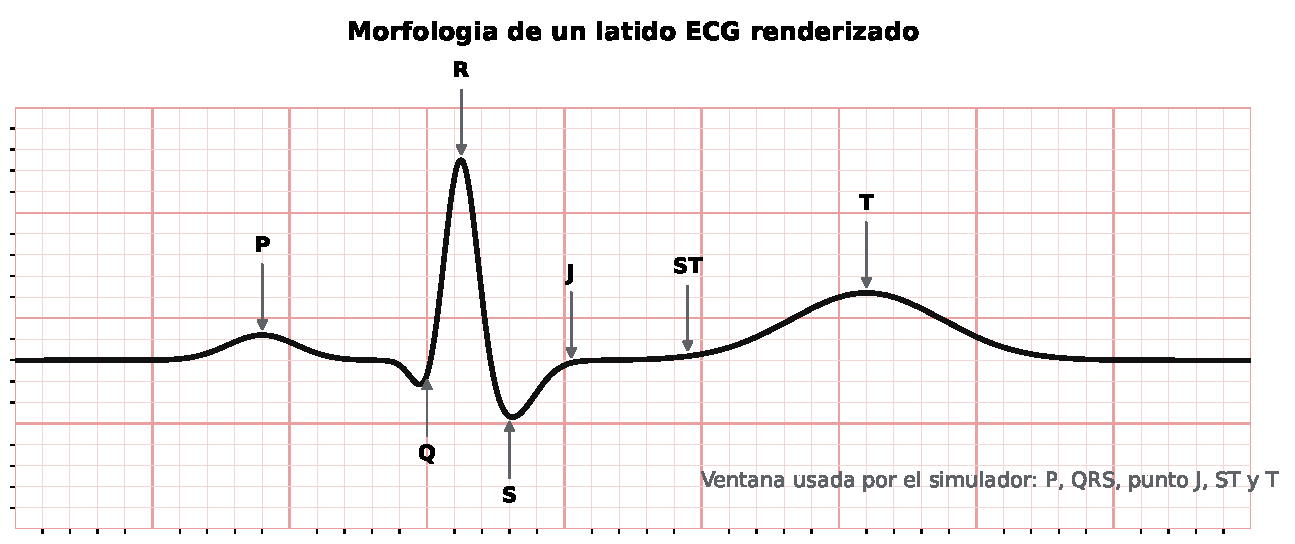
\includegraphics[trim=3bp 4bp 2bp 25bp,clip,width=226mm]{assets/fig_morfologia_ecg.pdf}\par
\vspace{4mm}
\begin{columns}[T,onlytextwidth]
\begin{column}{.34\textwidth}
{\color{UOGreen}\fontsize{20}{26}\selectfont Complejo QRS\par}
{\fontsize{16}{22}\selectfont Activación ventricular. El RBBB es un bloqueo de rama derecha que cambia la parte final del QRS.\par}
\end{column}
\begin{column}{.30\textwidth}
{\color{UOGreen}\fontsize{20}{26}\selectfont Segmento ST\par}
{\fontsize{16}{22}\selectfont Empieza en el punto J. Se observa si está elevado respecto a la línea de base.\par}
\end{column}
\begin{column}{.28\textwidth}
{\color{UOGreen}\fontsize{20}{26}\selectfont Onda T\par}
{\fontsize{16}{22}\selectfont Repolarización ventricular. Se observa si la onda está invertida.\par}
\end{column}
\end{columns}
\figurecaption{5}{Morfología de un latido y regiones de interés. Elaboración propia.}
\note{Leemos el trazado de izquierda a derecha. La P corresponde a la activación de las aurículas y el QRS, a la de los ventrículos. En el bloqueo de rama derecha, o RBBB, el ventrículo derecho se activa con retraso y puede aparecer una segunda deflexión positiva al final del QRS. En el simulador, RBBB etiqueta ese rasgo morfológico. Después del punto J miramos si el ST se eleva respecto a la línea de base y si la onda T, que corresponde a la repolarización ventricular, apunta hacia abajo.}
\end{frame}}

\expandafter\newcommand\csname Slidep03\endcsname{%
\renewcommand{\defenseblock}{Fundamentos clínicos}
\renewcommand{\defensenav}{Defensa del TFG}
\begin{frame}[c]\hypertarget{p03}{}
\frametitle{Síndrome de Brugada y derivación V1}
\begin{columns}[c,onlytextwidth]
\begin{column}{.63\textwidth}
\centering
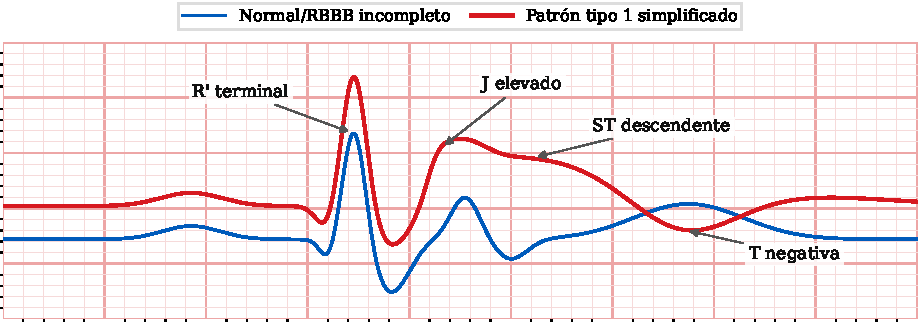
\includegraphics[width=\linewidth]{assets/fig_brugada_pattern.pdf}\par
\figurecaption{6}{Comparación esquemática del patrón de Brugada. Elaboración propia.}
\vspace{5mm}
{\fontsize{18}{24}\selectfont QRS terminal \quad --\quad Elevación del ST \quad --\quad Onda T negativa\par}
\end{column}
\begin{column}{.35\textwidth}
\centering
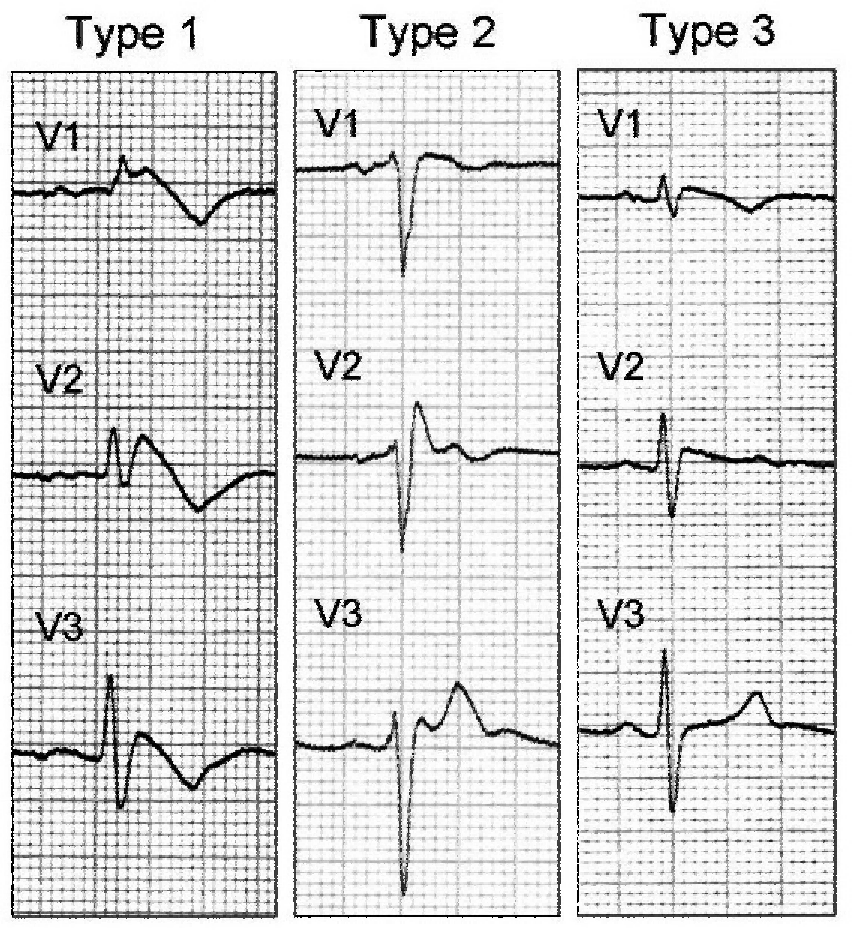
\includegraphics[width=\linewidth,height=101mm,keepaspectratio]{assets/brugada_patterns_orphanet.pdf}\par
\figurecaption{7}{Napolitano y Priori (2006), CC BY 2.0.}
\end{column}
\end{columns}
\note{La figura localiza en V1 las regiones que se examinan en un trazado sospechoso: el final del QRS, el ST y la onda T. En Brugada sus cambios pueden ser intermitentes, lo que añade dificultad a la hora de reunir ejemplos representativos de una enfermedad ya poco frecuente. La etiqueta clínica se asigna al paciente y puede incorporar información del ECG completo y de otras pruebas.}
\end{frame}}

\expandafter\newcommand\csname Slidea15\endcsname{%
\renewcommand{\defenseblock}{Fundamentos clínicos}
\renewcommand{\defensenav}{Defensa del TFG}
\begin{frame}[c]\hypertarget{a15}{}
\frametitle{Aspectos éticos y protección de datos}
\begin{columns}[t,onlytextwidth]
\begin{column}{.46\textwidth}
{\color{UOGreen}\rule{\linewidth}{1pt}}\par\vspace{5mm}
{\fontsize{26}{33}\selectfont Protección de los datos\par}
\vspace{6mm}
{\fontsize{20}{28}\selectfont Modelos de pesos abiertos para procesar los ECG sin enviarlos a servicios externos.\par}
\end{column}
\begin{column}{.46\textwidth}
{\color{UOGreen}\rule{\linewidth}{1pt}}\par\vspace{5mm}
{\fontsize{26}{33}\selectfont Responsabilidad clínica\par}
\vspace{6mm}
{\fontsize{20}{28}\selectfont Apoyo al triaje ante sospecha de síndrome de Brugada.\par}
\end{column}
\end{columns}
\note{El HUCA entregó los registros ya anonimizados. Los pesos abiertos de Gemma permitieron ejecutar la inferencia en un entorno privado. La posibilidad que se investiga es priorizar la revisión de ECG sospechosos bajo responsabilidad del personal sanitario.}
\end{frame}}

\expandafter\newcommand\csname Slidecnn_concepto\endcsname{%
\renewcommand{\defenseblock}{Fundamentos metodológicos}
\renewcommand{\defensenav}{Defensa del TFG}
\begin{frame}[c]\hypertarget{cnn_concepto}{}
\frametitle{Redes neuronales convolucionales}
\centering
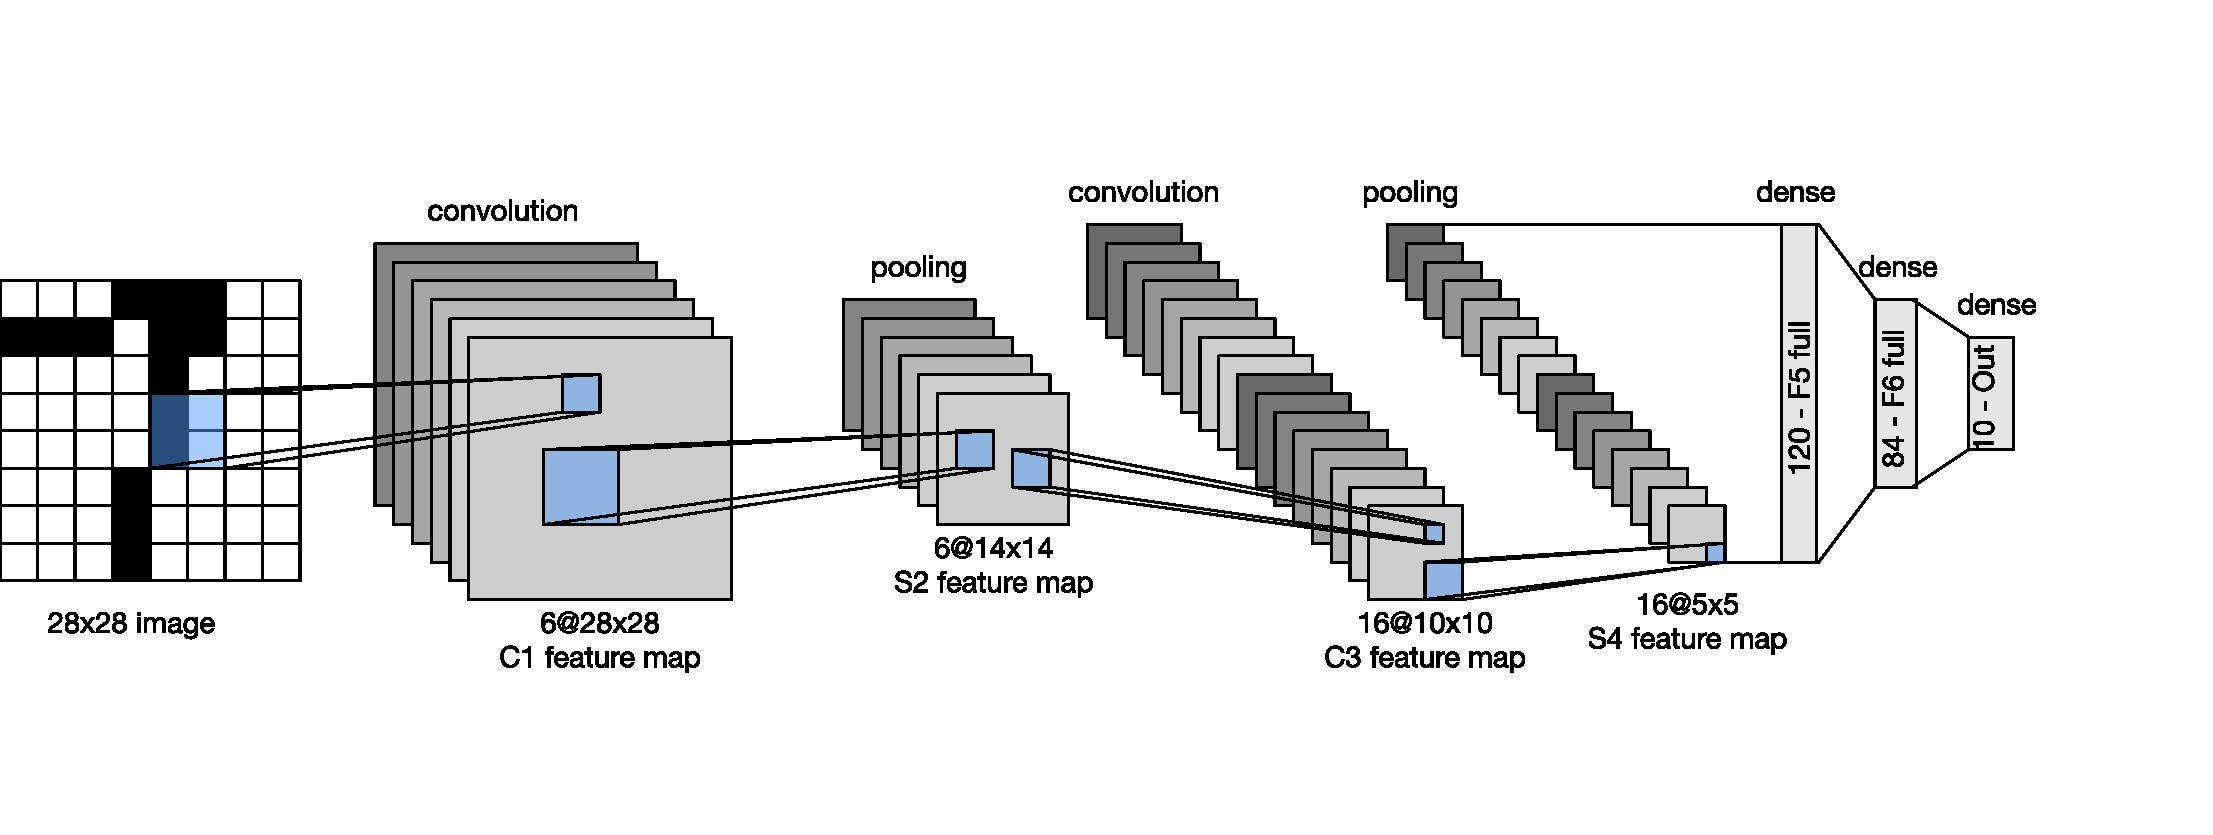
\includegraphics[trim=0 55bp 60bp 65bp,clip,width=267mm,height=86mm,keepaspectratio]{assets/referencias_visuales/lenet.pdf}\par
\vspace{4mm}
\begin{columns}[t,onlytextwidth]
\begin{column}{.31\textwidth}\centering
{\color{UOGreen}\fontsize{23}{30}\selectfont Convolución\par}
{\fontsize{17}{23}\selectfont Aplica filtros a la imagen\par}
\end{column}
\begin{column}{.31\textwidth}\centering
{\color{UOGreen}\fontsize{23}{30}\selectfont \textit{Pooling}\par}
{\fontsize{17}{23}\selectfont Reduce la resolución espacial\par}
\end{column}
\begin{column}{.31\textwidth}\centering
{\color{UOGreen}\fontsize{23}{30}\selectfont Clasificación\par}
{\fontsize{17}{23}\selectfont Predice la clase\par}
\end{column}
\end{columns}
\vspace{3mm}
\figurecaption{8}{\href{https://commons.wikimedia.org/wiki/File:LeNet-5_architecture.svg}{Arquitectura LeNet-5, Zhang y colaboradores. Dive into Deep Learning (CC BY-SA 4.0).}}
\note{Una convolución recorre la imagen con filtros cuyos coeficientes aprende la red. Un filtro puede resaltar, por ejemplo, los bordes del trazado. El pooling resume las activaciones y reduce su resolución espacial. La capa de clasificación usa esas características para producir una predicción. Durante el entrenamiento, el error respecto a las etiquetas guía el ajuste de los pesos.}
\end{frame}}

\expandafter\newcommand\csname Slidep05\endcsname{%
\renewcommand{\defenseblock}{Datos y simulación}
\renewcommand{\defensenav}{Defensa del TFG}
\begin{frame}[c]\hypertarget{p05}{}
\frametitle{Conjuntos de datos del simulador y del HUCA}
\begin{columns}[T,onlytextwidth]
\begin{column}{.47\textwidth}\centering
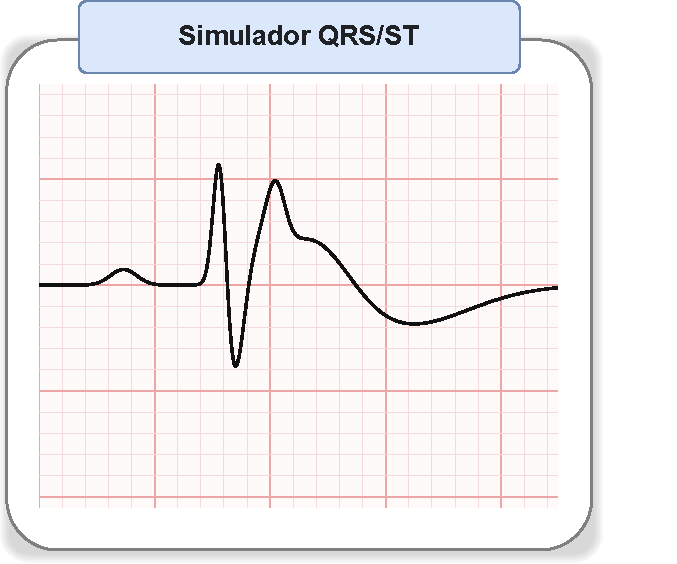
\includegraphics[width=\linewidth,height=91mm,keepaspectratio]{assets/comparison_simulator_panel.pdf}\par
\vspace{3mm}
{\fontsize{22}{29}\selectfont\SimPatients{} casos, \SimPositive{} positivos\par}
\figurecaption{9}{Trazado del simulador QRS/ST. Elaboración propia.}
\end{column}
\begin{column}{.47\textwidth}\centering
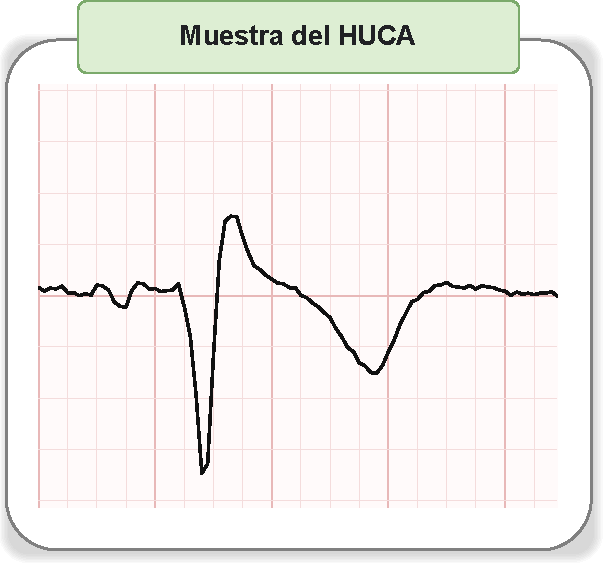
\includegraphics[width=\linewidth,height=91mm,keepaspectratio]{assets/comparison_huca_panel.pdf}\par
\vspace{3mm}
{\fontsize{22}{29}\selectfont\HucaPatients{} pacientes, \HucaPositive{} positivos\par}
\figurecaption{10}{Trazado renderizado del HUCA. Elaboración propia.}
\end{column}
\end{columns}
\note{Los dos conjuntos aportan imágenes de un latido de V1. El simulador genera \SimPatients{} casos y sus etiquetas describen rasgos morfológicos. El HUCA aporta \HucaPatients{} pacientes con una etiqueta clínica por persona. Los trazados que se muestran son ejemplos independientes.}
\end{frame}}

\expandafter\newcommand\csname Slidep06\endcsname{%
\renewcommand{\defenseblock}{Datos y simulación}
\renewcommand{\defensenav}{Defensa del TFG}
\begin{frame}[c]\hypertarget{p06}{}
\frametitle{Simulador QRS/ST}
\fullfigure[109mm]{gaussian_generator.drawio.pdf}
\takeaway{El latido se construye como suma de gaussianas.}
\figurecaption{11}{Simulador QRS/ST mediante componentes gaussianas. Elaboración propia, basado en Sayadi et al. (2010).}
\note{El simulador construye cada latido sumando gaussianas. Su amplitud, posición y anchura permiten modificar regiones de las ondas. Sayadi y colaboradores utilizaron componentes gaussianos en un modelo dinámico. El simulador de este trabajo suma directamente los componentes. Las etiquetas se asignan a partir de los rasgos que aparecen en el latido generado.}
\end{frame}}

\expandafter\newcommand\csname Slidea04\endcsname{%
\renewcommand{\defenseblock}{Datos y simulación}
\renewcommand{\defensenav}{Defensa del TFG}
\begin{frame}[c]\hypertarget{a04}{}
\frametitle{Familias del simulador}
\fullfigure[108mm]{fig_synthetic_examples.pdf}
\figurecaption{12}{Familias de trazados del simulador QRS/ST. Elaboración propia.}
\note{Las familias incluyen un trazado de referencia y distintas combinaciones de cambios en el QRS, el ST y la onda T. Cada familia permite generar ejemplos con una morfología distinta.}
\end{frame}}

\expandafter\newcommand\csname Slidehuca\endcsname{%
\renewcommand{\defenseblock}{Datos y simulación}
\renewcommand{\defensenav}{Defensa del TFG}
\begin{frame}[c]\hypertarget{huca}{}
\frametitle{Conjunto clínico del HUCA}
\begin{columns}[c,onlytextwidth]
\begin{column}{.55\textwidth}
\centering
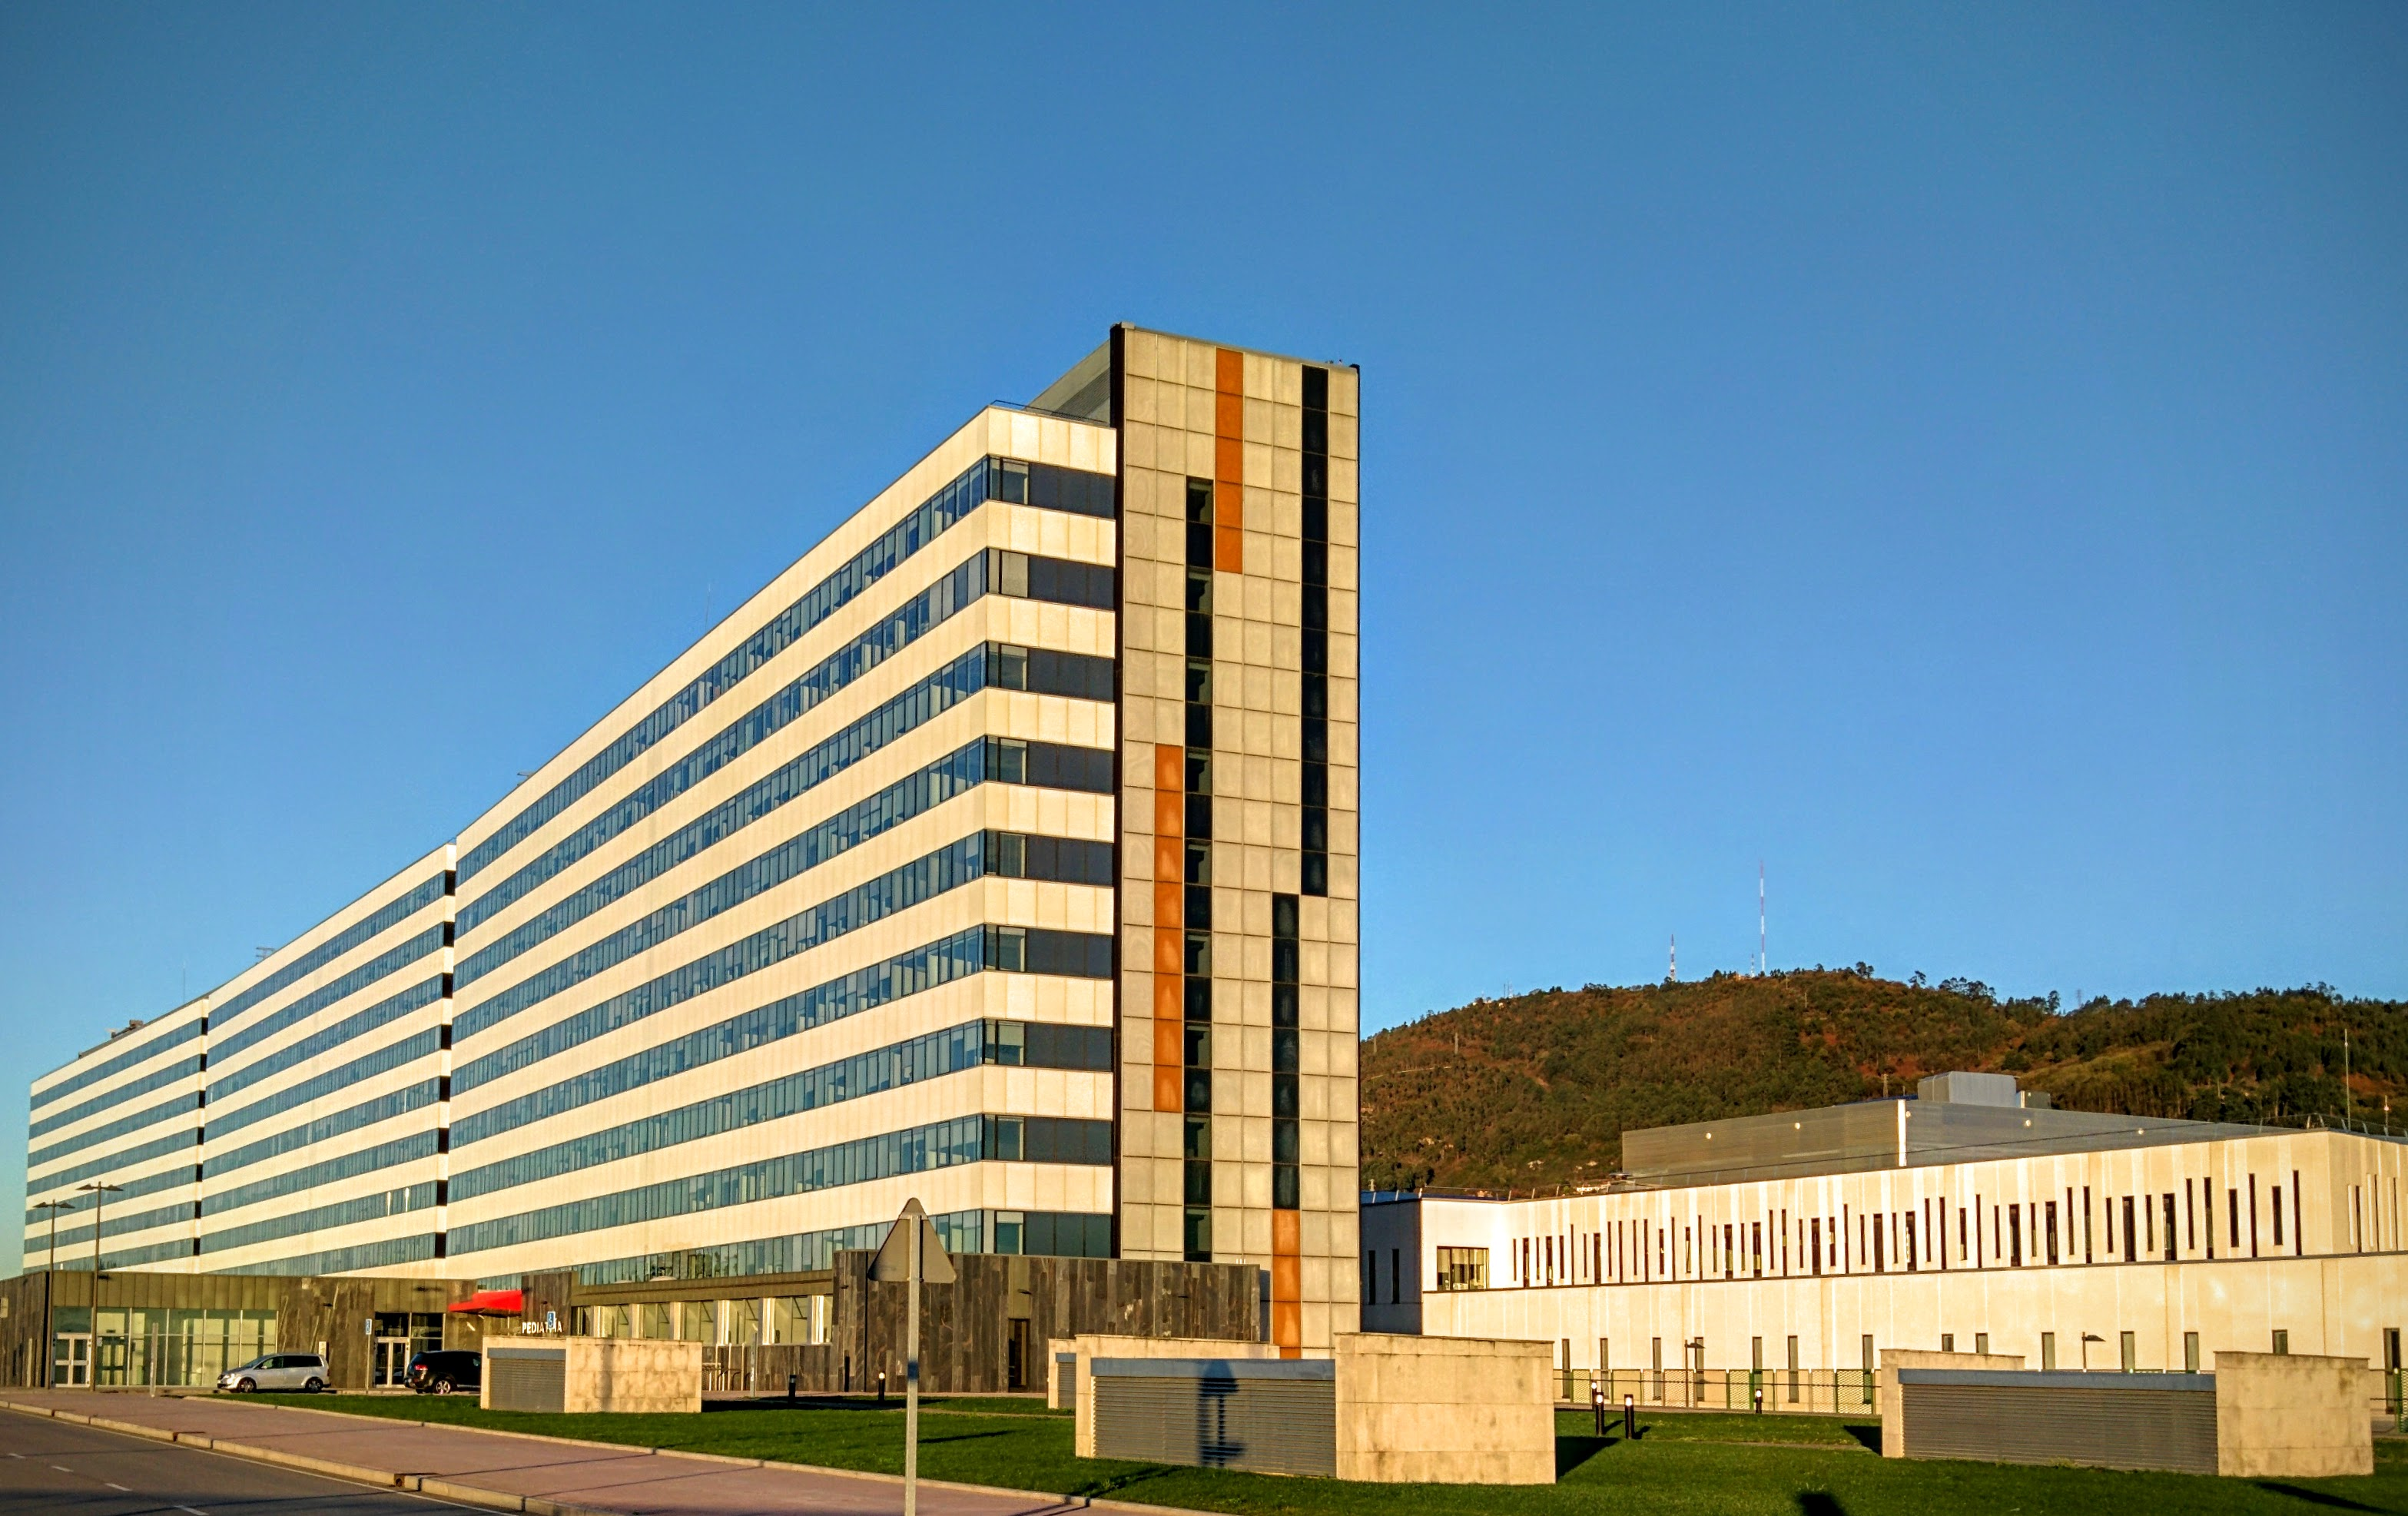
\includegraphics[width=\linewidth,height=100mm,keepaspectratio]{assets/referencias_visuales/huca.jpg}\par
\figurecaption{13}{\href{https://commons.wikimedia.org/wiki/File:HUCA.jpg}{Hospital Universitario Central de Asturias. LMLM, Wikimedia Commons (CC BY-SA 4.0).}}
\end{column}
\begin{column}{.41\textwidth}
{\color{UOGreen}\fontsize{45}{52}\selectfont\HucaPatients{}}\enspace{\fontsize{23}{30}\selectfont pacientes}\par
\vspace{4mm}
{\fontsize{19}{26}\selectfont\HucaPositive{} con etiqueta positiva\par
\HucaNegative{} con etiqueta negativa\par}
\vspace{8mm}
{\color{UOGreen}\fontsize{23}{30}\selectfont Selección de casos\par}
{\fontsize{19}{26}\selectfont Se excluyeron 46 casos dudosos.\par}
\end{column}
\end{columns}
\note{La campaña evaluó \HucaPatients{} pacientes, con \HucaPositive{} etiquetas positivas y \HucaNegative{} negativas. Según la memoria, se excluyeron casos que los colaboradores clínicos aconsejaron dejar fuera por dudas de clasificación. En el código, los 46 casos excluidos son los que tenían a la vez la etiqueta positiva de Brugada y el indicador de patrón basal patológico en la copia de trabajo. La copia pública de PhysioNet tiene etiquetas distintas. Los recuentos de la diapositiva corresponden a la muestra utilizada en el TFG. La evaluación emplea las etiquetas de la copia de trabajo. Algunas difieren de los metadatos de la publicación de PhysioNet.}
\end{frame}}

\expandafter\newcommand\csname Slidep04\endcsname{%
\renewcommand{\defenseblock}{Diseño experimental}
\renewcommand{\defensenav}{Defensa del TFG}
\begin{frame}[c]\hypertarget{p04}{}
\frametitle{Diseño experimental}
\fullfigure[108mm]{fig_pipeline_experimental.pdf}
\figurecaption{14}{Diseño experimental de VLM/ICL y CNN. Elaboración propia.}
\note{El esquema muestra dos formas de utilizar los ECG etiquetados. Empiezo por Gemma: las demostraciones forman parte de la consulta y el modelo clasifica con sus pesos fijos. En la otra rama, ResNet18 ajusta sus pesos antes de clasificar un ECG nuevo. A la derecha se resume cómo se evalúan los dos enfoques.}
\end{frame}}

\expandafter\newcommand\csname Slidep08\endcsname{%
\renewcommand{\defenseblock}{Implementación}
\renewcommand{\defensenav}{Defensa del TFG}
\begin{frame}[c]\hypertarget{p08}{}
\frametitle{Implementación del ICL con Gemma 4 E4B}
\fullfigure[108mm]{vlm_icl_context_window.pdf}
\figurecaption{15}{Clasificación mediante aprendizaje en contexto con pesos fijos. Elaboración propia.}
\note{E4B es una variante compacta de la familia Gemma 4 de Google. La consulta contiene instrucciones, demostraciones etiquetadas y la imagen que se quiere clasificar. Se prueban selecciones estándar y balanceadas por clase. El modelo devuelve etiquetas estructuradas para calcular las métricas.}
\end{frame}}

\expandafter\newcommand\csname Slidep07\endcsname{%
\renewcommand{\defenseblock}{Implementación}
\renewcommand{\defensenav}{Defensa del TFG}
\begin{frame}[c]\hypertarget{p07}{}
\frametitle{Implementación de la CNN con ResNet18}
\fullfigure[108mm]{cnn_convolutional_pipeline.pdf}
\figurecaption{16}{Entrenamiento y predicción de la CNN ResNet18. Elaboración propia.}
\note{La CNN utiliza ResNet18 preentrenada y ajusta la red completa. La imagen se convierte a gris, se redimensiona y se replica su intensidad en tres canales para respetar la entrada de ResNet18. El simulador requiere tres salidas morfológicas. El entrenamiento con HUCA utiliza una salida para la etiqueta clínica.}
\end{frame}}

\expandafter\newcommand\csname Slidea06\endcsname{%
\renewcommand{\defenseblock}{Implementación}
\renewcommand{\defensenav}{Defensa del TFG}
\begin{frame}[c]\hypertarget{a06}{}
\frametitle{Superposición de Grad-CAM sobre ECG}
\centering
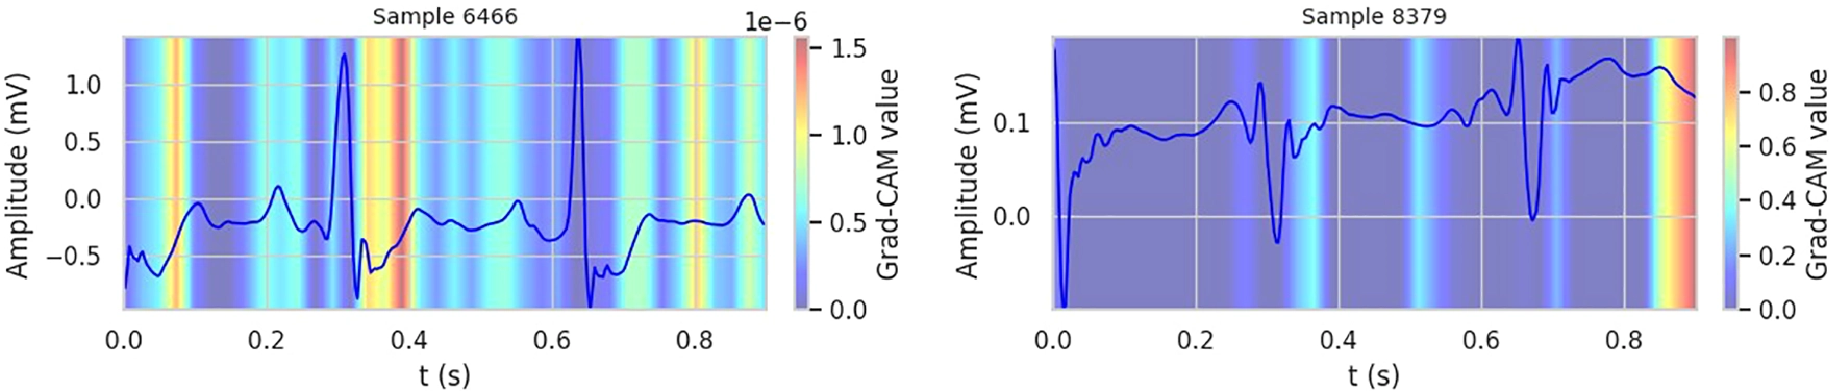
\includegraphics[width=282mm]{assets/gradcam_ecg_published_example.pdf}\par
\vspace{7mm}
{\fontsize{22}{29}\selectfont El color sitúa las regiones que más contribuyen a la salida del modelo.\par}
\vspace{3mm}
\figurecaption{17}{Ejemplos publicados de Grad-CAM sobre ECG. \href{https://doi.org/10.3389/fphys.2026.1848316}{Sundaramoorthy y Karunanidhi (2026)}, CC BY 4.0. Recorte.}
\note{Esta figura publicada ilustra la superposición de Grad-CAM sobre una señal de ECG. Los colores cálidos corresponden a valores mayores del mapa dentro de cada ejemplo, según su escala. La activación indica una contribución relativa a la salida del modelo y no demuestra por sí sola una interpretación clínica correcta. Es una ilustración bibliográfica de un clasificador de arritmias sobre señales, no un resultado de la CNN de este TFG ni un ejemplo de Brugada. En nuestro estudio, Grad-CAM se aplicó a imágenes de un latido central de V1. Fuente: \href{https://doi.org/10.3389/fphys.2026.1848316}{Sundaramoorthy y Karunanidhi (2026)}, figura 15, recortada a la fila superior, CC BY 4.0.}
\end{frame}}

\expandafter\newcommand\csname Slideescenarios\endcsname{%
\renewcommand{\defenseblock}{Diseño experimental}
\renewcommand{\defensenav}{Defensa del TFG}
\begin{frame}[c]\hypertarget{escenarios}{}
\frametitle{Escenarios de evaluación}
\centering
{\fontsize{22}{30}\selectfont
\setlength{\tabcolsep}{4mm}
\renewcommand{\arraystretch}{1.55}
\begin{tabular}{@{}p{90mm}p{104mm}p{80mm}@{}}
\toprule
\scenarioheading
\midrule
\hyperlink{escenario_simulador}{\textcolor{UOGray}{01}\enspace Simulación} & Simulador & Simulador\\
\hyperlink{escenario_transferencia}{\textcolor{UOGray}{02}\enspace Cambio de dominio} & Simulador & HUCA\\
\hyperlink{escenario_clinico}{\textcolor{UOGray}{03}\enspace Evaluación clínica} & HUCA & HUCA\\
\bottomrule
\end{tabular}\par}
\note{Primero se evalúan los dos enfoques dentro del simulador. Después se mantienen los ejemplos simulados y se pasa a evaluar en el HUCA, donde también se prueban estrategias de adaptación. Por último, tanto los ejemplos como la evaluación proceden del HUCA.}
\end{frame}}

\expandafter\newcommand\csname Slidep09\endcsname{%
\renewcommand{\defenseblock}{Diseño experimental}
\renewcommand{\defensenav}{Defensa del TFG}
\begin{frame}[c]\hypertarget{p09}{}
\frametitle{Protocolo de evaluación por paciente: LOOCV}
\fullfigure[108mm]{clinical_fold_protocol.pdf}
\figurecaption{18}{Protocolo LOOCV por paciente. Elaboración propia.}
\note{K es el número de demostraciones para Gemma o casos de entrenamiento para ResNet18. Se evalúan cinco valores con tres semillas. Cada pliegue reserva un paciente para la prueba. La CNN clínica dispone además de ocho pacientes de validación para elegir época y umbral.}
\end{frame}}

\expandafter\newcommand\csname Slidemetricas\endcsname{%
\renewcommand{\defenseblock}{Diseño experimental}
\renewcommand{\defensenav}{Defensa del TFG}
\begin{frame}[c]\hypertarget{metricas}{}
\frametitle{Métricas de evaluación}
\begin{columns}[T,onlytextwidth]
\begin{column}{.53\textwidth}
{\fontsize{17}{23}\selectfont
\setlength{\tabcolsep}{3mm}
\renewcommand{\arraystretch}{1.1}
\begin{tabular}{@{}p{25mm}p{52mm}p{52mm}@{}}
& \multicolumn{2}{c}{\textcolor{UOGray}{Predicción del modelo}}\\[2mm]
& \centering Positivo & \centering Negativo\tabularnewline[3mm]
\textcolor{UOGray}{Positivo real}
& \cellcolor{UOGreen!12}\rule{0pt}{12mm}{\fontsize{27}{32}\selectfont\color{UOGreen} VP}\par\vspace{2mm}Positivo detectado\par\vspace{5mm}
& \cellcolor{ScenarioRed!12}\rule{0pt}{12mm}{\fontsize{27}{32}\selectfont\color{ScenarioRed} FN}\par\vspace{2mm}Caso omitido\par\vspace{5mm}\tabularnewline[2mm]
\textcolor{UOGray}{Negativo real}
& \cellcolor{ScenarioRed!12}\rule{0pt}{12mm}{\fontsize{27}{32}\selectfont\color{ScenarioRed} FP}\par\vspace{2mm}Falsa alarma\par\vspace{5mm}
& \cellcolor{UOGreen!12}\rule{0pt}{12mm}{\fontsize{27}{32}\selectfont\color{UOGreen} VN}\par\vspace{2mm}Negativo descartado\par\vspace{5mm}\tabularnewline
\end{tabular}\par}
\end{column}
\begin{column}{.41\textwidth}
{\fontsize{27}{34}\selectfont\color{UOGreen} BA\enspace {\fontsize{19}{26}\selectfont Exactitud balanceada}\par}
\vspace{3mm}
{\fontsize{22}{29}\selectfont Cada clase pesa un 50\%.\par}
\vspace{3mm}
{\fontsize{16}{23}\selectfont Sensibilidad: positivos detectados.\\Especificidad: negativos descartados.\par}
\vspace{2mm}
{\fontsize{16}{23}\selectfont La clase mayoritaria no domina.\par}
\vspace{7mm}
{\fontsize{27}{34}\selectfont\color{UOGreen} F1\enspace {\fontsize{19}{26}\selectfont Clase positiva}\par}
\vspace{3mm}
{\fontsize{21}{28}\selectfont Combina sensibilidad y precisión.\par}
\vspace{3mm}
{\fontsize{16}{23}\selectfont Precisión: aciertos entre los señalados.\par}
\end{column}
\end{columns}
\vspace{6mm}
{\color{UOLine}\hrule height0.5pt}
\vspace{4mm}
{\fontsize{18}{25}\selectfont\color{UOGreen} Triaje\enspace {\color{UOInk} Reducir casos omitidos y controlar las falsas alarmas.}\par}
\figurecaption{19}{Matriz de confusión conceptual y métricas binarias. Elaboración propia. Definiciones de scikit-learn.}
\note{La exactitud global puede parecer alta si predominan los negativos y el modelo casi siempre predice esa clase. La exactitud balanceada promedia sensibilidad y especificidad, por lo que cada clase pesa lo mismo aunque sus tamaños difieran. La sensibilidad es la proporción de positivos de referencia que se detectan. Un falso negativo es un positivo de referencia que el modelo clasifica como negativo. La especificidad es la proporción de negativos de referencia que se descartan. Un falso positivo es un negativo que se señala como positivo.

F1 se calcula para la clase positiva y es la media armónica de precisión y sensibilidad. La precisión indica cuántos de los casos señalados son positivos según la referencia. F1 disminuye cuando se acumulan falsos positivos o falsos negativos, pero no incluye los verdaderos negativos y no asigna por sí sola un mayor coste clínico a omitir un caso. Tampoco la exactitud balanceada expresa la utilidad clínica de los errores: da el mismo peso a la sensibilidad y la especificidad, no un coste asistencial acordado.

Como posible apoyo al triaje, interesa reducir los falsos negativos para no dejar casos sospechosos sin priorizar, controlando a la vez los falsos positivos porque aumentan las revisiones. La importancia relativa de los errores depende del uso y debe acordarse con especialistas y validarse. Una BA o una F1 altas no bastan para afirmar que el sistema puede descartar pacientes. Por eso se presentan también sensibilidad, especificidad y matrices de confusión. Esta explicación no modifica umbrales ni el protocolo experimental.

En la evaluación del HUCA, positivo se refiere a la etiqueta clínica empleada. En el simulador, la clase derivada procede de las reglas morfológicas QRS/ST. Son objetivos de anotación distintos y no se convierten en diagnósticos clínicos intercambiables. Las fórmulas son las mismas para cada tarea binaria, pero se interpretan respecto a su propia referencia.

Fuentes: \href{https://scikit-learn.org/stable/modules/generated/sklearn.metrics.balanced_accuracy_score.html}{scikit-learn: exactitud balanceada}. \href{https://scikit-learn.org/stable/modules/generated/sklearn.metrics.f1_score.html}{F1}. \href{https://scikit-learn.org/stable/modules/generated/sklearn.metrics.recall_score.html}{sensibilidad o recall}. \href{https://scikit-learn.org/stable/modules/generated/sklearn.metrics.precision_score.html}{precisión}.

La matriz de confusión de esta diapositiva es un esquema conceptual sin recuentos, no un resultado experimental. Las filas son la etiqueta de referencia y las columnas la predicción. La diagonal representa los aciertos. Las celdas fuera de la diagonal distinguen casos omitidos y falsas alarmas. BA equivale a la media de sensibilidad y especificidad. Al dar un cincuenta por ciento a cada clase, aumenta el peso relativo de la minoritaria respecto a la exactitud global. F1 equivale a dos veces VP dividido entre dos veces VP más FP más FN. Combina precisión y sensibilidad mediante su media armónica. Las fórmulas se conservan en las notas para dejar la diapositiva como apoyo visual.}
\end{frame}}

\expandafter\newcommand\csname Slideescenario_simulador\endcsname{%
\renewcommand{\defenseblock}{Resultados}
\renewcommand{\defensenav}{Defensa del TFG}
\begin{frame}[plain]\hypertarget{escenario_simulador}{}
\scenariofocus{Simulación}{Simulador}{Simulador}
\note{En el primer escenario, los ejemplos y los datos de prueba son simulados.}
\end{frame}}

\expandafter\newcommand\csname Slidep10\endcsname{%
\renewcommand{\defenseblock}{Resultados 1/3 \enspace Simulador \(\rightarrow\) Simulador}
\renewcommand{\defensenav}{Defensa del TFG}
\begin{frame}[c]\hypertarget{p10}{}
\frametitle{Resultados con ejemplos del simulador}
\begin{columns}[c,onlytextwidth]
\begin{column}{.49\textwidth}\centering
\begin{minipage}[c][92mm][c]{\linewidth}\centering
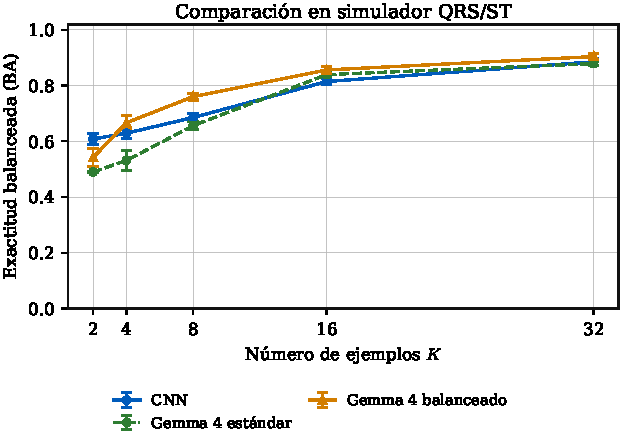
\includegraphics[width=\linewidth,height=92mm,keepaspectratio]{assets/comparison_simulator_ba_by_k.pdf}
\end{minipage}\par
\figurecaption{20}{Exactitud balanceada en el simulador. Elaboración propia.}
\end{column}
\begin{column}{.49\textwidth}\centering
\begin{minipage}[c][92mm][c]{\linewidth}\centering
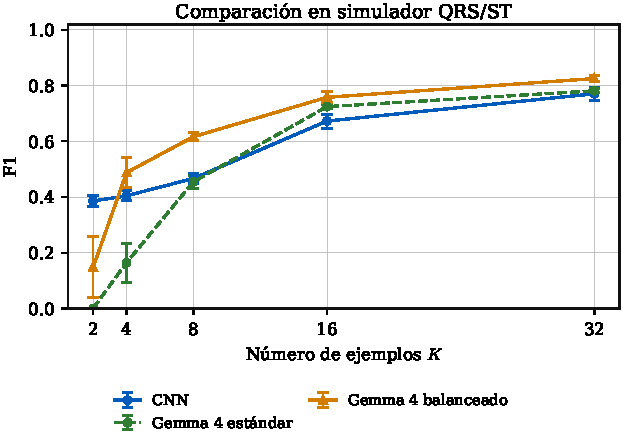
\includegraphics[width=\linewidth,height=92mm,keepaspectratio]{assets/comparison_simulator_f1_by_k.pdf}
\end{minipage}\par
\figurecaption{21}{F1 en el simulador. Elaboración propia.}
\end{column}
\end{columns}
\note{El eje horizontal indica el número de ejemplos. Gemma, con demostraciones balanceadas, llega a una exactitud balanceada de \SimVlmBA{}. La referencia ResNet18 llega a \SimCnnBA{}. Ambos métodos mejoran a medida que aumenta el número de ejemplos. Las barras muestran la desviación estándar entre tres semillas. F1 resume la precisión y la sensibilidad de la clase positiva.}
\end{frame}}

\expandafter\newcommand\csname Slidea07\endcsname{%
\renewcommand{\defenseblock}{Resultados 1/3 \enspace Simulador \(\rightarrow\) Simulador}
\renewcommand{\defensenav}{Defensa del TFG}
\begin{frame}[c]\hypertarget{a07}{}
\frametitle{Matrices de confusión en el simulador}
\begin{columns}[c,onlytextwidth]
\begin{column}{.49\textwidth}\centering
\begin{minipage}[c][92mm][c]{\linewidth}\centering
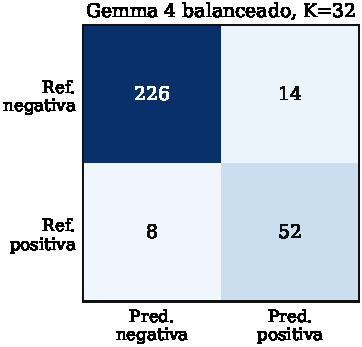
\includegraphics[width=\linewidth,height=92mm,keepaspectratio]{assets/vlm_simulator_qrs_balanced_k32_confusion_matrix.pdf}
\end{minipage}\par
\figurecaption{22}{Matriz de confusión de Gemma. Elaboración propia.}
\end{column}
\begin{column}{.49\textwidth}\centering
\begin{minipage}[c][92mm][c]{\linewidth}\centering
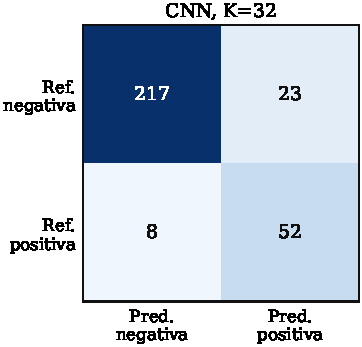
\includegraphics[width=\linewidth,height=92mm,keepaspectratio]{assets/cnn_simulator_qrs_k32_confusion_matrix.pdf}
\end{minipage}\par
\figurecaption{23}{Matriz de confusión de la CNN. Elaboración propia.}
\end{column}
\end{columns}
\note{A la izquierda se ve Gemma con 32 demostraciones balanceadas y a la derecha ResNet18 con el mismo número de ejemplos de entrenamiento. Las filas separan positivos y negativos reales. Gemma genera menos falsos positivos en esta comparación. Cada matriz reúne tres evaluaciones sobre los mismos casos.}
\end{frame}}

\expandafter\newcommand\csname Slideescenario_transferencia\endcsname{%
\renewcommand{\defenseblock}{Resultados}
\renewcommand{\defensenav}{Defensa del TFG}
\begin{frame}[plain]\hypertarget{escenario_transferencia}{}
\scenariofocus{Cambio de dominio}{Simulador}{HUCA}
\note{En el segundo escenario se mantienen los ejemplos simulados y se evalúa en el HUCA.}
\end{frame}}

\expandafter\newcommand\csname Slideantecedente_dominio\endcsname{%
\renewcommand{\defenseblock}{Resultados 2/3 \enspace Simulador \(\rightarrow\) HUCA}
\renewcommand{\defensenav}{Defensa del TFG}
\begin{frame}[c]\hypertarget{antecedente_dominio}{}
\frametitle{Adaptación de dominio}
\centering
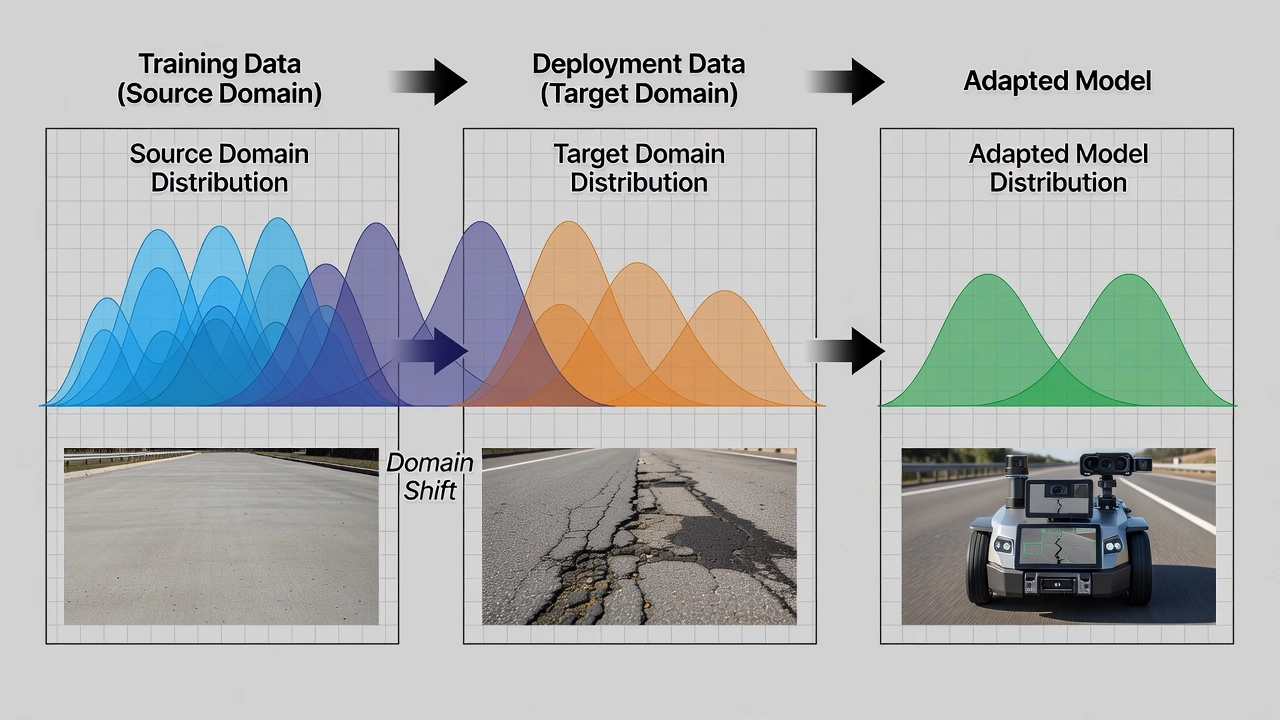
\includegraphics[width=260mm,height=104mm,keepaspectratio]{assets/referencias_visuales/tarmac_domain.png}\par
\vspace{2mm}
{\fontsize{18}{24}\selectfont Simulador \(\rightarrow\) HUCA\par}
\figurecaption{24}{\href{https://www.tarmacview.com/es/glossary/domain-adaptation/}{Fuente de la ilustración: TarmacView, glosario de adaptación de dominio.}}
\note{La ilustración muestra qué significa entrenar con imágenes de un origen y evaluar con imágenes de otro. Aquí pasamos de latidos simulados a registros del HUCA. Cambian el aspecto del trazado y la etiqueta evaluada: primero se describen rasgos de un latido y después se clasifica al paciente. En la CNN se probó incorporar imágenes del HUCA sin sus etiquetas para reducir la diferencia visual.}
\end{frame}}

\expandafter\newcommand\csname Slidea11\endcsname{%
\renewcommand{\defenseblock}{Resultados 2/3 \enspace Simulador \(\rightarrow\) HUCA}
\renewcommand{\defensenav}{Defensa del TFG}
\begin{frame}[c]\hypertarget{a11}{}
\frametitle{Cambio de dominio en ICL con selección estándar}
\centering
\definecolor{ICLSynthetic}{HTML}{2E7D32}
\definecolor{ICLClinical}{HTML}{75B978}
\definecolor{ICLTransfer}{HTML}{666666}
{\fontsize{14}{19}\selectfont
\begin{tikzpicture}[baseline=-.5ex]\draw[ICLSynthetic,line width=1.15pt] (0,0)--(.65,0);\fill[ICLSynthetic] (.325,0) circle[radius=1.3pt];\end{tikzpicture}\enspace Simulador \quad
\begin{tikzpicture}[baseline=-.5ex]\draw[ICLClinical,dashed,line width=1.15pt] (0,0)--(.65,0);\fill[ICLClinical] (.325,0) circle[radius=1.3pt];\end{tikzpicture}\enspace HUCA, contexto HUCA \quad
\begin{tikzpicture}[baseline=-.5ex]\draw[ICLTransfer,dotted,line width=1.15pt] (0,0)--(.65,0);\fill[ICLTransfer] (.325,0) circle[radius=1.3pt];\end{tikzpicture}\enspace HUCA, contexto del simulador\par}
\vspace{3mm}
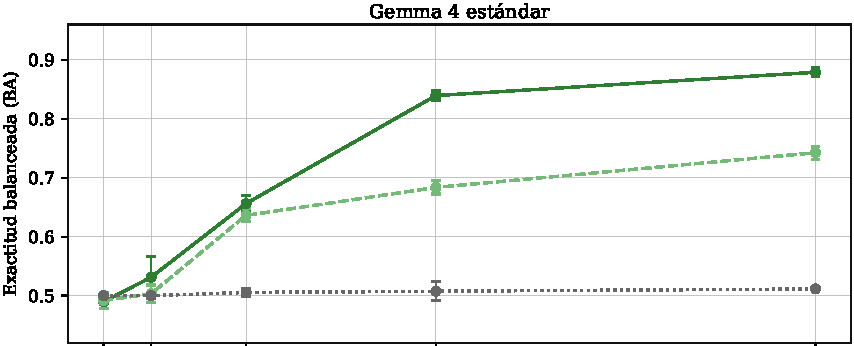
\includegraphics[width=245mm]{assets/context_standard.pdf}\par
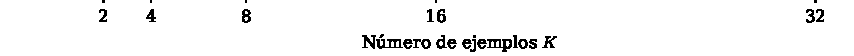
\includegraphics[width=245mm]{assets/context_xaxis.pdf}\par
\figurecaption{25}{Efecto del origen de los ejemplos con selección estándar. Elaboración propia.}
\note{Con selección estándar, se compara el efecto del origen de las demostraciones. Las consultas clínicas se benefician de ejemplos del HUCA, mientras que las demostraciones simuladas aportan poco al clasificar los registros clínicos.}
\end{frame}}

\expandafter\newcommand\csname Slidep11\endcsname{%
\renewcommand{\defenseblock}{Resultados 2/3 \enspace Simulador \(\rightarrow\) HUCA}
\renewcommand{\defensenav}{Defensa del TFG}
\begin{frame}[c]\hypertarget{p11}{}
\frametitle{CNN entrenada en el simulador y evaluada en el HUCA}
\fullfigure[108mm]{domain_gap_cnn_ba_by_k.pdf}
\figurecaption{26}{Evaluación de la CNN ante el cambio de dominio. Elaboración propia.}
\note{Aquí se entrena la CNN con datos del simulador y se cambia el conjunto de prueba. La línea continua representa la evaluación simulada y la discontinua, la clínica. Con treinta y dos ejemplos la exactitud balanceada clínica queda en \TransferCnnLastBA{}. El cambio de dominio afecta tanto al aspecto del trazado como a las etiquetas.}
\end{frame}}

\expandafter\newcommand\csname Slidea09\endcsname{%
\renewcommand{\defenseblock}{Resultados 2/3 \enspace Simulador \(\rightarrow\) HUCA}
\renewcommand{\defensenav}{Defensa del TFG}
\begin{frame}[c]\hypertarget{a09}{}
\frametitle{Métodos de adaptación de dominio en la CNN}
\centering
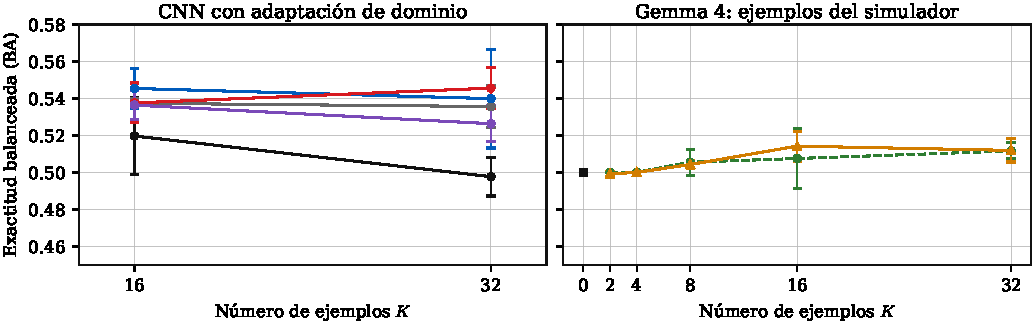
\includegraphics[width=257mm]{assets/transfer_ba.pdf}\par

\includegraphics[width=257mm]{assets/transfer_legend.pdf}\par
\figurecaption{27}{Exactitud balanceada de las variantes de adaptación. Elaboración propia.}
\note{Gemma con demostraciones sintéticas aparece en el panel derecho. En la izquierda, la comparación muestra las cuatro variantes de adaptación de la CNN. Usan imágenes clínicas sin sus etiquetas, incluidas las que se evalúan después. CORAL y MMD mejoran algunos puntos frente a ResNet18 con el mismo K. La mejor exactitud balanceada global sigue correspondiendo a la referencia sin adaptación.}
\end{frame}}

\expandafter\newcommand\csname Slidea10\endcsname{%
\renewcommand{\defenseblock}{Resultados 2/3 \enspace Simulador \(\rightarrow\) HUCA}
\renewcommand{\defensenav}{Defensa del TFG}
\begin{frame}[c]\hypertarget{a10}{}
\frametitle{F1 de la clase positiva al cambiar de dominio}
\fullfigure[108mm]{transfer_f1.pdf}
\figurecaption{28}{F1 de la clase positiva ante el cambio de dominio. Elaboración propia.}
\note{El panel de F1 permite examinar la detección de positivos al cambiar de dominio. El rendimiento sigue siendo bajo en la clasificación clínica, tanto con las variantes de adaptación como con las demostraciones simuladas de Gemma. Esto ayuda a interpretar una especificidad alta cuando se predice casi siempre la clase negativa.}
\end{frame}}

\expandafter\newcommand\csname Slideescenario_clinico\endcsname{%
\renewcommand{\defenseblock}{Resultados}
\renewcommand{\defensenav}{Defensa del TFG}
\begin{frame}[plain]\hypertarget{escenario_clinico}{}
\scenariofocus{Evaluación clínica}{HUCA}{HUCA}
\note{En el tercer escenario, tanto los ejemplos como la prueba proceden del HUCA.}
\end{frame}}

\expandafter\newcommand\csname Slidep13\endcsname{%
\renewcommand{\defenseblock}{Resultados 3/3 \enspace HUCA \(\rightarrow\) HUCA}
\renewcommand{\defensenav}{Defensa del TFG}
\begin{frame}[c]\hypertarget{p13}{}
\frametitle{Demostraciones y entrenamiento con ejemplos del HUCA}
\centering

\includegraphics[width=178mm]{assets/clinical_legend.pdf}\par
\begin{columns}[T,onlytextwidth]
\begin{column}{.49\textwidth}
\centering
{\fontsize{19}{26}\selectfont Exactitud balanceada\par}
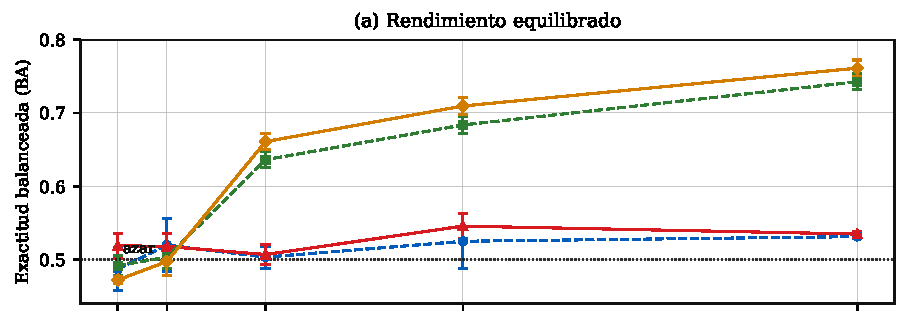
\includegraphics[width=\linewidth,trim=0 0 0 15bp,clip]{assets/clinical_ba.pdf}\par
\vspace{-1mm}
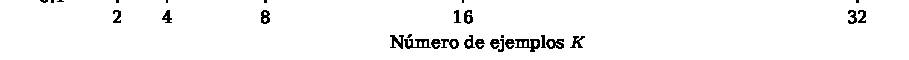
\includegraphics[width=\linewidth,trim=0 0 0 3bp,clip]{assets/clinical_xaxis.pdf}\par
\end{column}
\begin{column}{.49\textwidth}
\centering
{\fontsize{19}{26}\selectfont F1 de la clase positiva\par}
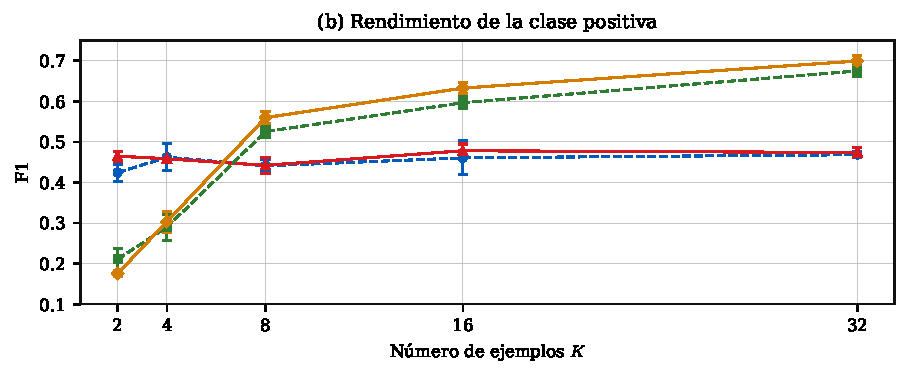
\includegraphics[width=\linewidth,trim=0 0 0 15bp,clip]{assets/clinical_f1.pdf}\par
\end{column}
\end{columns}
\takeaway{Con \(K=32\), la exactitud balanceada es \RealVlmBA{} para Gemma y \RealCnnLastBA{} para la CNN en selección balanceada.}
\figurecaption{29}{Exactitud balanceada y F1 con ejemplos clínicos del HUCA. Elaboración propia.}
\note{En el tercer escenario, Gemma recibe demostraciones del HUCA y ResNet18 se entrena con imágenes del mismo conjunto. El paciente de prueba queda reservado en ambos casos. A la izquierda vemos la exactitud balanceada. A la derecha se muestra F1 para la clase positiva. F1 baja cuando el modelo deja casos positivos sin detectar o cuando da demasiadas falsas alarmas. Sin demostraciones, Gemma no resulta capaz de identificar positivos en la evaluación realizada. Con dos o cuatro ejemplos, la mejor CNN conserva una ligera ventaja. Desde ocho ejemplos, Gemma con selección balanceada obtiene mejores resultados. Con treinta y dos alcanza una exactitud balanceada de \RealVlmBA{}, frente a \RealCnnLastBA{} de la CNN balanceada, y un F1 de \RealVlmFone{}. La comparación se refiere a esta muestra y a las configuraciones evaluadas.}
\end{frame}}

\expandafter\newcommand\csname Slidep14\endcsname{%
\renewcommand{\defenseblock}{Resultados 3/3 \enspace HUCA \(\rightarrow\) HUCA}
\renewcommand{\defensenav}{Defensa del TFG}
\begin{frame}[c]\hypertarget{p14}{}
\frametitle{Matrices de confusión en la evaluación clínica}
\fullfigure[108mm]{clinical_cnn_vs_gemma_confusions.pdf}
\figurecaption{30}{Matrices de confusión en la evaluación clínica. Elaboración propia.}
\note{Las matrices muestran las mejores configuraciones balanceadas de cada método. A la izquierda, Gemma utiliza treinta y dos demostraciones. A la derecha, ResNet18 utiliza dieciséis ejemplos de entrenamiento. Gemma obtiene una sensibilidad de \RealVlmSens{} y una especificidad de \RealVlmSpec{}. Esto deja sin identificar alrededor de una cuarta parte de los positivos. Las matrices se normalizan por clase real y agregan tres evaluaciones de los mismos pacientes.}
\end{frame}}

\expandafter\newcommand\csname Slidep16\endcsname{%
\renewcommand{\defenseblock}{Conclusiones y discusión}
\renewcommand{\defensenav}{Defensa del TFG}
\begin{frame}[c]\hypertarget{p16}{}
\frametitle{Conclusiones}
\begin{columns}[t,onlytextwidth]

\begin{column}{.31\textwidth}
{\color{UOGreen}\rule{\linewidth}{1.15pt}}\par\vspace{4mm}
{\fontsize{22}{29}\selectfont Comparación en el HUCA\par}
\vspace{9mm}
\begin{minipage}[t]{.48\linewidth}
{\color{UOGreen}\fontsize{35}{43}\selectfont\strut\RealVlmBA{}\par}
{\fontsize{17}{22}\selectfont Gemma\par}
\end{minipage}\hfill
\begin{minipage}[t]{.48\linewidth}
{\color{UOGreen}\fontsize{35}{43}\selectfont\strut\RealCnnLastBA{}\par}
{\fontsize{17}{22}\selectfont CNN\par}
\end{minipage}\par\vspace{3mm}
{\fontsize{18}{26}\selectfont Exactitud balanceada con 32 ejemplos del HUCA y selección balanceada.\par}
\end{column}
\begin{column}{.31\textwidth}
{\color{UOGreen}\rule{\linewidth}{1.15pt}}\par\vspace{4mm}
{\fontsize{22}{29}\selectfont Número de ejemplos\par}
\vspace{9mm}
{\color{UOGreen}\fontsize{32}{43}\selectfont Mejora en ambos\par}
\vspace{3mm}
{\fontsize{18}{26}\selectfont En el simulador, ambos métodos mejoran al disponer de más ejemplos etiquetados.\par}
\end{column}
\begin{column}{.31\textwidth}
{\color{UOGreen}\rule{\linewidth}{1.15pt}}\par\vspace{4mm}
{\fontsize{22}{29}\selectfont Transferencia al HUCA\par}
\vspace{9mm}
{\color{UOGreen}\fontsize{35}{43}\selectfont\TransferCnnLastBA{}\par}
\vspace{3mm}
{\fontsize{18}{26}\selectfont Exactitud balanceada en el HUCA de la CNN entrenada con 32 ejemplos simulados.\par}
\end{column}
\end{columns}
\note{Con ejemplos del HUCA, Gemma supera a ResNet18 desde ocho demostraciones. Con 32 y selección balanceada, la exactitud balanceada es \RealVlmBA{} para Gemma y \RealCnnLastBA{} para ResNet18. El simulador demuestra que ambos aprovechan más ejemplos en una tarea controlada. Al usar ejemplos sintéticos sobre el HUCA el rendimiento cae, lo que pone de relieve la importancia de la procedencia de las demostraciones.}
\end{frame}}

\expandafter\newcommand\csname Slidep15\endcsname{%
\renewcommand{\defenseblock}{Conclusiones y discusión}
\renewcommand{\defensenav}{Defensa del TFG}
\begin{frame}[c]\hypertarget{p15}{}
\frametitle{Limitaciones del estudio}
\begin{columns}[T,onlytextwidth]
\begin{column}{.47\textwidth}
\begin{minipage}[c][70mm][c]{\linewidth}
\centering
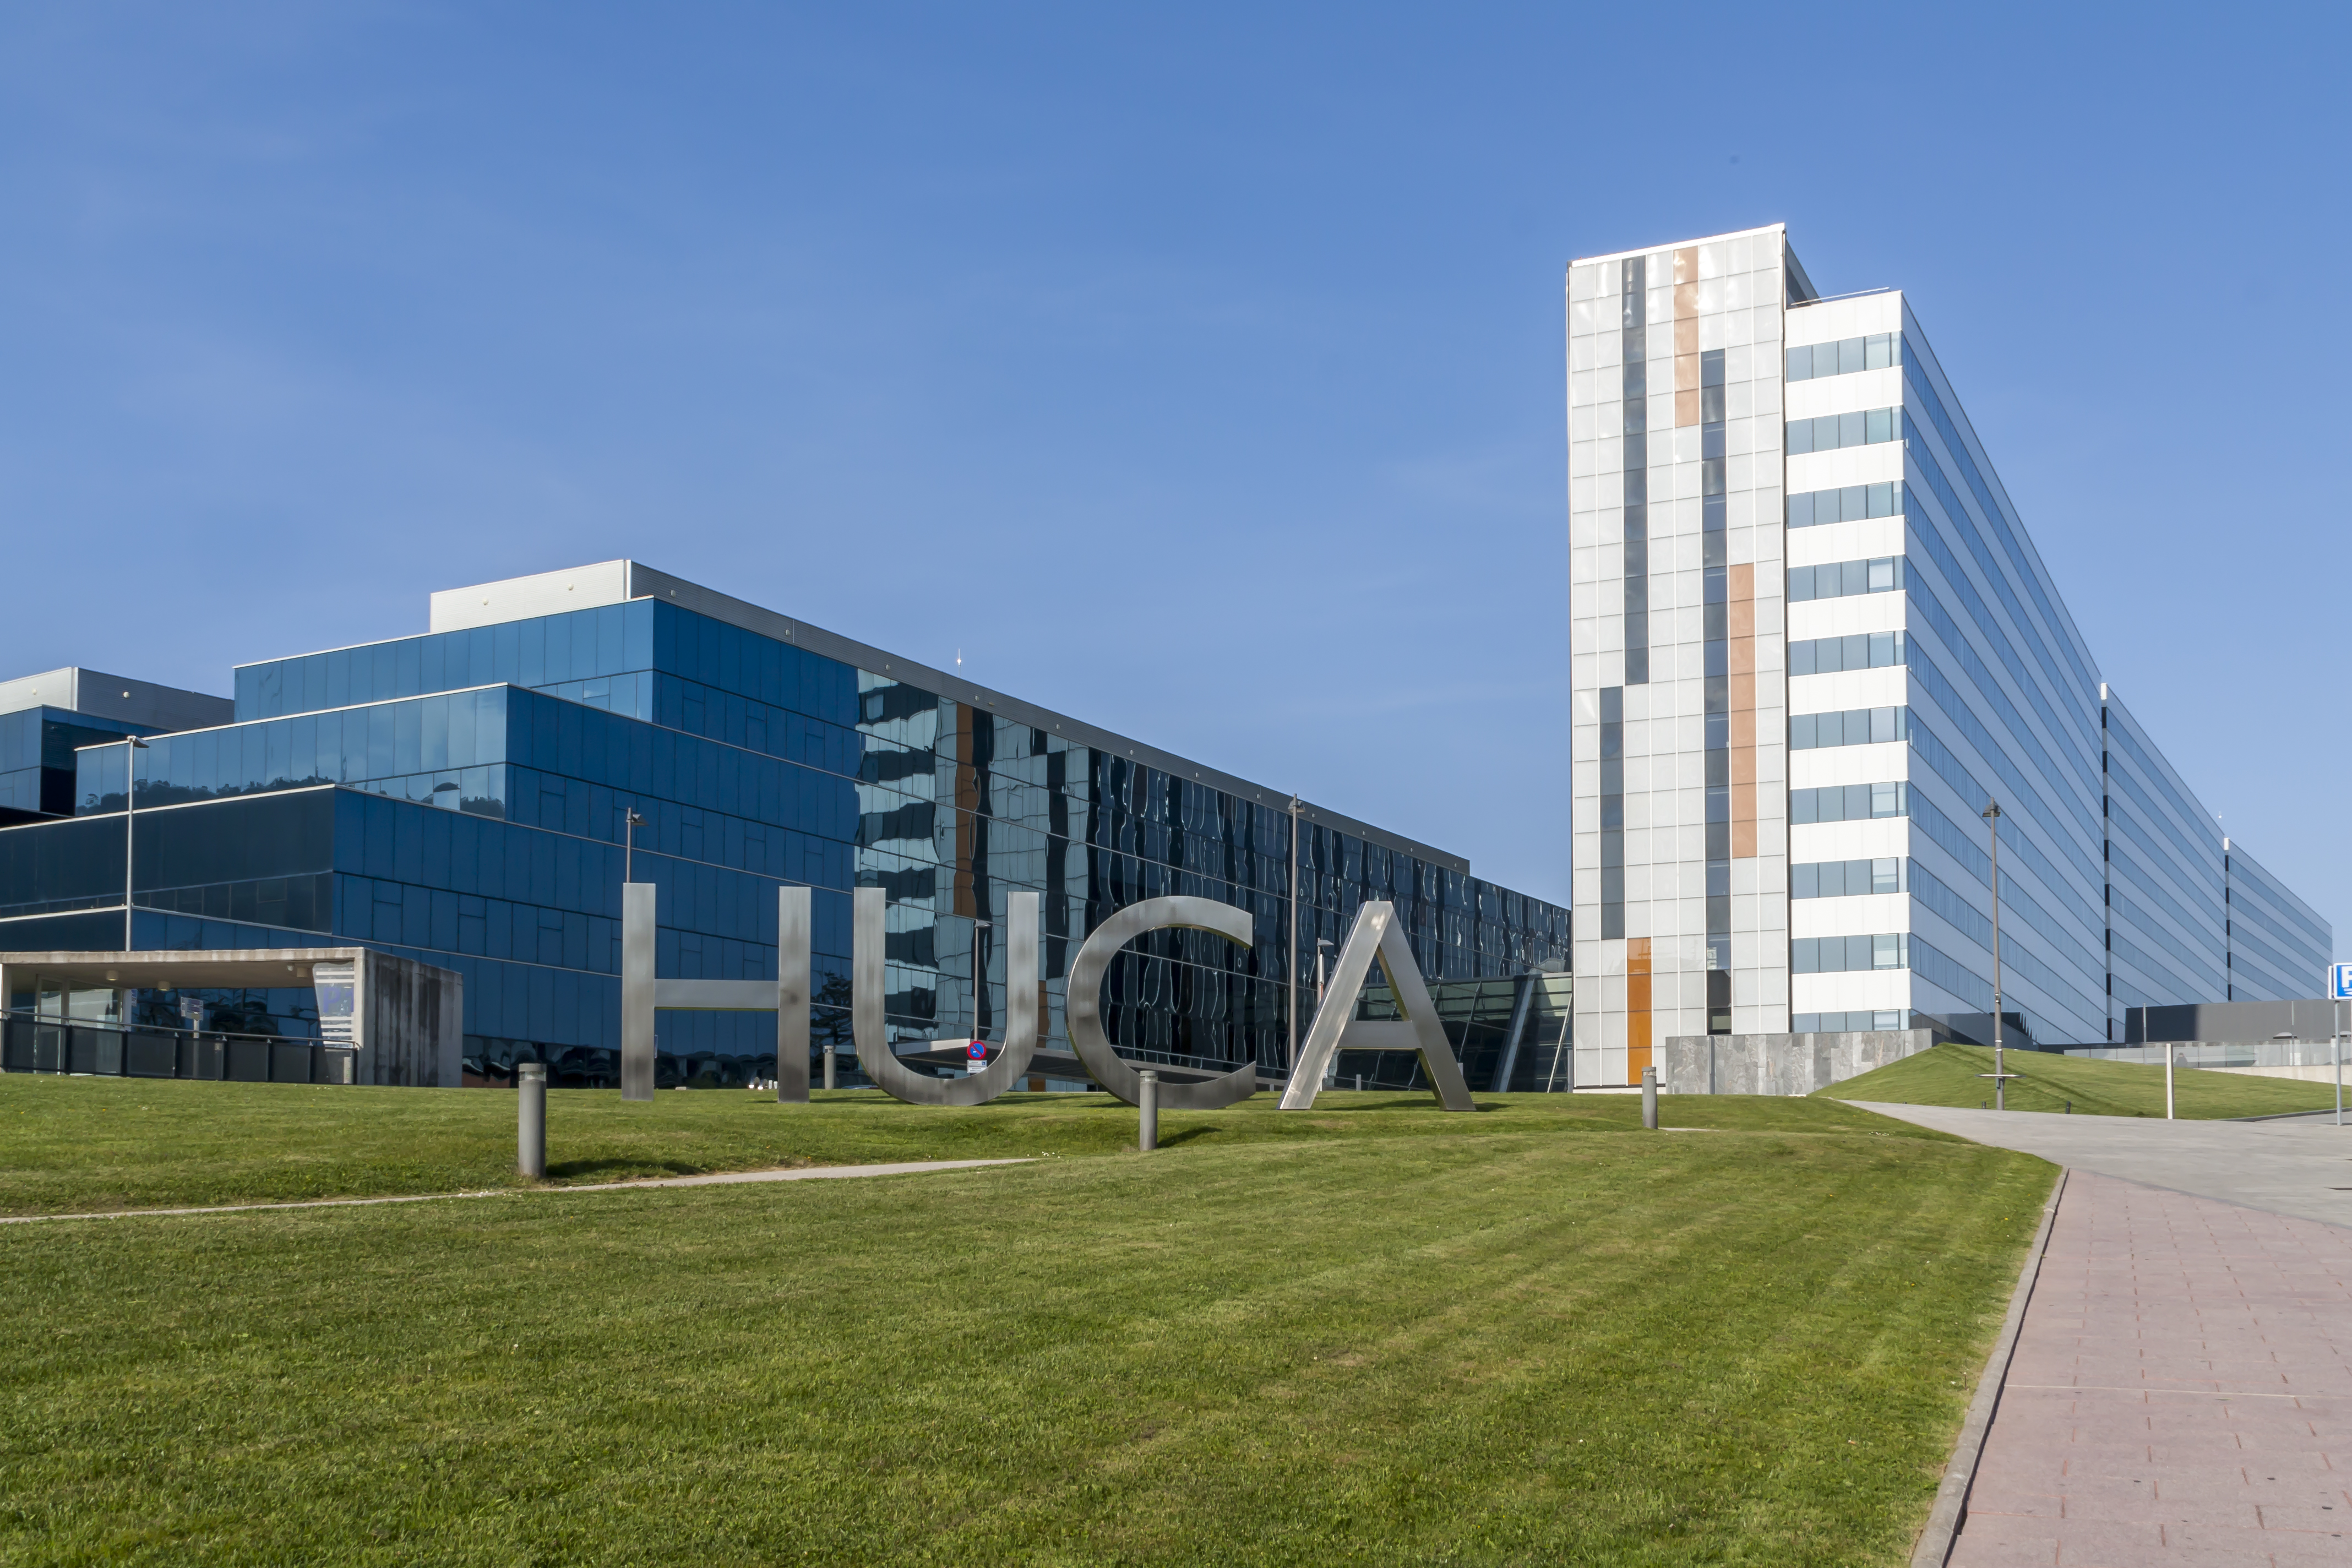
\includegraphics[trim=0bp 110bp 0bp 80bp,clip,width=\linewidth,height=70mm,keepaspectratio]{assets/referencias_visuales/huca_vicenmiranda.jpg}
\end{minipage}\par
\vspace{5mm}
{\fontsize{22}{29}\selectfont\color{UOGreen} Muestra de un único hospital\par}
\vspace{3mm}
{\fontsize{18}{25}\selectfont\HucaPatients{} pacientes del HUCA.\\Muestra limitada, sin validación externa.\par}
\end{column}
\begin{column}{.47\textwidth}
\begin{minipage}[c][70mm][c]{\linewidth}
\centering
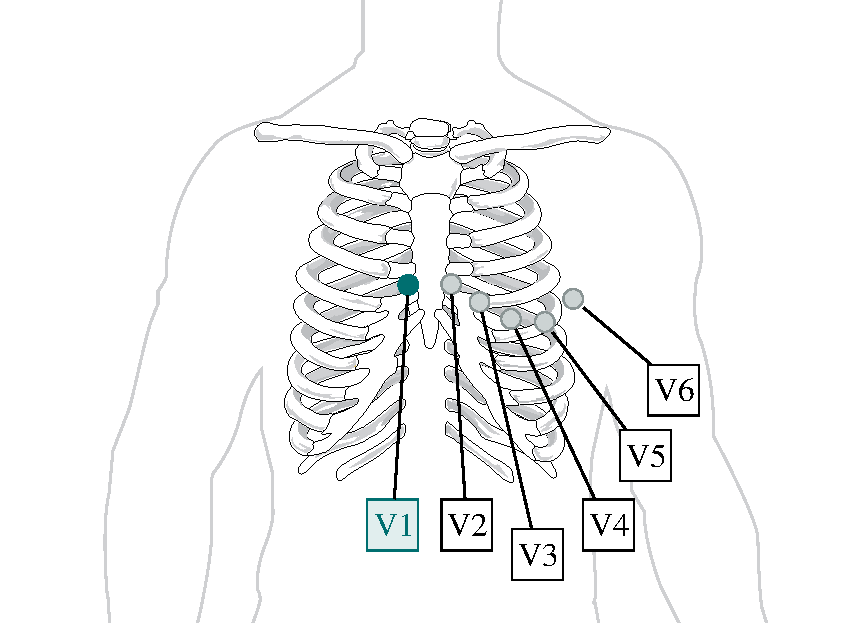
\includegraphics[width=\linewidth,height=70mm,keepaspectratio]{assets/referencias_visuales/precordial_v1_highlight.pdf}
\end{minipage}\par
\vspace{5mm}
{\fontsize{22}{29}\selectfont\color{UOGreen} Un latido de la derivación V1\par}
\vspace{3mm}
{\fontsize{18}{25}\selectfont V1 es una derivación precordial.\\Representación parcial del ECG.\par}
\end{column}
\end{columns}
\vspace{5mm}
\figurecaption{31}{Fotografía: \href{https://commons.wikimedia.org/wiki/File:25._Hospital_Universitario_Central_de_Asturias_(36104132056).jpg}{vicenmiranda, CC BY 2.0, recorte}. Esquema precordial: \href{https://commons.wikimedia.org/wiki/File:Precordial_Leads.svg}{Twisp, dominio público. V1 resaltada}.}
\note{Las limitaciones se concentran en la procedencia de la muestra y en la representación de entrada. La evaluación clínica utiliza \HucaPatients{} pacientes del Hospital Universitario Central de Asturias. Aunque permite comparar los métodos dentro de esta cohorte, su tamaño y la escasez de ejemplos positivos limitan la variedad de trazados y etiquetas observada. Todos los pacientes proceden del mismo hospital. No se ha validado el rendimiento en una cohorte externa. Por tanto, estos resultados no establecen la generalización a otros hospitales o poblaciones.

La entrada es un trazado renderizado de un latido central de la derivación precordial V1. No se utiliza el registro temporal completo ni la información conjunta de las doce derivaciones. Esta selección reduce la información disponible y acota el alcance del experimento a esa representación. La ilustración muestra la disposición de las derivaciones precordiales y destaca V1. No representa un paciente ni un resultado del estudio.

La fotografía del HUCA es de vicenmiranda, publicada en Wikimedia Commons con licencia CC BY 2.0. Se recorta para la composición. El esquema anatómico es de Twisp y está en dominio público. En la adaptación se elimina el fondo azul y se resalta V1 con la paleta de la defensa, conservando la disposición anatómica. Las fuentes y licencias se conservan en la documentación de los recursos visuales. La adaptación de dominio y la ampliación de datos se abordan en la diapositiva de trabajo futuro.}
\end{frame}}

\expandafter\newcommand\csname Slidefuturo\endcsname{%
\renewcommand{\defenseblock}{Conclusiones y discusión}
\renewcommand{\defensenav}{Defensa del TFG}
\begin{frame}[c]\hypertarget{futuro}{}
\frametitle{Continuación del trabajo}
{\fontsize{23}{31}\selectfont
\begin{tabular}{@{}p{17mm}l@{}}
\textcolor{UOGreen}{01} & Revisar las etiquetas y ampliar su recogida\\[7mm]
\textcolor{UOGreen}{02} & Explorar otros rasgos morfológicos del ECG\\[7mm]
\textcolor{UOGreen}{03} & Explorar otros métodos de adaptación de dominio\\[7mm]
\textcolor{UOGreen}{04} & Validar el apoyo al triaje en el HUCA y después en otros centros
\end{tabular}}
\note{La continuación empieza por revisar las etiquetas con especialistas y ampliar la recogida de casos etiquetados. Se estudiarían otros rasgos morfológicos del ECG y se probarían otros métodos de adaptación de dominio. Por último, se evaluaría si el sistema ayuda a priorizar ECG sospechosos en el HUCA y después en otros centros sanitarios.}
\end{frame}}

\expandafter\newcommand\csname Slidecierre\endcsname{%
\renewcommand{\defenseblock}{}
\renewcommand{\defensenav}{Defensa del TFG}
\begin{frame}[plain]\hypertarget{cierre}{}
\hypertarget{conclusion}{}
\begin{tikzpicture}[remember picture,overlay]
\node[anchor=north,inner sep=0pt] at ([yshift=-18mm]current page.north) {
\includegraphics[height=30mm]{assets/logo_uniovi_portada.pdf}};
\node[anchor=center,text=UOInk] at ([yshift=8mm]current page.center) {\fontsize{32}{40}\selectfont Gracias por su atención};
\node[anchor=center,text=UOInk] at ([yshift=-9mm]current page.center) {\fontsize{19}{25}\selectfont Preguntas};
\node[anchor=center,text=UOInk] at ([yshift=-25mm]current page.center) {\fontsize{21}{27}\selectfont\AuthorName};
\node[anchor=south west,inner sep=0pt] at ([xshift=15mm,yshift=5mm]current page.south west) {
\includegraphics[height=9mm]{assets/logo_epi_horizontal.pdf}};
\node[anchor=south east,inner sep=0pt,text=UOInk] at ([xshift=-15mm,yshift=5mm]current page.south east) {\fontsize{17}{22}\selectfont\SubmissionDate};
\end{tikzpicture}
\note{Gracias por su atención. Quedo a disposición del tribunal para las preguntas.}
\end{frame}}

\expandafter\newcommand\csname Slidepresupuesto\endcsname{%
\renewcommand{\defenseblock}{Presupuesto}
\renewcommand{\defensenav}{Defensa del TFG}
\begin{frame}[c]\hypertarget{presupuesto}{}
\frametitle{Presupuesto aproximado}
\begin{columns}[T,onlytextwidth]
\begin{column}{.54\textwidth}
{\fontsize{22}{28}\selectfont\color{UOGreen} Personal\par}
\vspace{3mm}
{\fontsize{16}{22}\selectfont
\renewcommand{\arraystretch}{.95}
\begin{tabular}{@{}p{75mm}p{49mm}r@{}}
Concepto & Dedicación & Coste\\\midrule
Investigación y desarrollo & 300 h $\times$ 20 €/h & 6.000 €\\[2mm]
Tutoría docente & 40 h $\times$ 50 €/h & 2.000 €\\[2mm]
Asesoramiento clínico & 10 h $\times$ 60 €/h & 600 €\\\midrule
\textbf{Subtotal personal} & & \textbf{8.600 €}\\
\end{tabular}\par}
\end{column}
\begin{column}{.42\textwidth}
{\fontsize{22}{28}\selectfont\color{UOGreen} Cómputo\par}
\vspace{3mm}
{\fontsize{16}{22}\selectfont
\renewcommand{\arraystretch}{.85}
\begin{tabular}{@{}p{44mm}p{48mm}r@{}}
2 A100 & 20 h, uso y luz & 51 €\\
RTX 3060 & 10 h, electricidad & 1 €\\\midrule
\textbf{Subtotal} & & \textbf{52 €}\\
\end{tabular}\par}
\vspace{3mm}
{\fontsize{22}{28}\selectfont\color{UOGreen} Materiales y servicios\par}
\vspace{3mm}
{\fontsize{16}{22}\selectfont
\renewcommand{\arraystretch}{.85}
\begin{tabular}{@{}p{95mm}r@{}}
Equipo amortizado & 150 €\\
Almacenamiento y copias & 30 €\\
Software libre & 0 €\\\midrule
\textbf{Subtotal} & \textbf{180 €}\\
\end{tabular}\par}
\end{column}
\end{columns}
\vspace{3mm}
{\color{UOLine}\hrule height0.5pt}
\vspace{3mm}
\begin{columns}[c,onlytextwidth]
\begin{column}{.55\textwidth}
{\fontsize{17}{23}\selectfont Base: 8.832 €\quad +\quad Imprevistos (10\%): 883 €\par}
\end{column}
\begin{column}{.41\textwidth}
{\fontsize{17}{23}\selectfont\color{UOGreen} Total estimado\par}
{\fontsize{29}{35}\selectfont 9.715 €\enspace {\fontsize{15}{21}\selectfont $\approx$ 9.700 €}\par}
\end{column}
\end{columns}
\vspace{3mm}
{\fontsize{14}{20}\selectfont\color{UOGreen} Tiempos registrados: Gemma 8,34 h de consultas. CNN 2,83 h de entrenamiento.\par}
\note{El presupuesto valora de forma aproximada el personal y los recursos del estudio. La estructura sigue la sección 6.2, página 72, del TFG de Nahuel Costa Cortez de 2019, sin reutilizar sus precios históricos. Las dedicaciones y tarifas del personal son hipótesis de cálculo. Se mantienen trescientas horas de investigación a veinte euros, cuarenta horas de tutoría a cincuenta euros y diez horas de asesoramiento clínico a sesenta euros.

Según la información del autor, Gemma se ejecutó en un clúster autogestionado cedido por su tutor con dos A100. La CNN se entrenó en su propio ordenador con una RTX 3060. No se presupone una factura de alquiler en la nube. La capacidad y el formato de las A100 no están confirmados. Como escenario de valoración se usa un precio de reposición redondeado de siete mil quinientos euros por A100, próximo al anuncio público de HydraGPU para una A100 de ochenta gigabytes reacondicionada a siete mil cuatrocientos setenta y nueve euros. Es una referencia comercial actual, no el precio pagado por las tarjetas utilizadas.

Se añaden tres mil euros supuestos para el resto del nodo. Dieciocho mil euros amortizados en cuatro años y dos mil horas productivas por año equivalen a dos euros con veinticinco céntimos por hora del nodo completo, con las dos GPU. Para veinte horas se imputan cuarenta y cinco euros. Ese coste es una valoración del recurso cedido, no un pago del estudiante. La utilización anual y la vida útil son supuestos que influyen en el resultado.

La ficha de NVIDIA sitúa el TDP máximo por A100 entre doscientos cincuenta y cuatrocientos vatios según la variante. Se considera de forma conservadora un kilovatio para las dos GPU y el resto del nodo, un factor de refrigeración de uno con dos y una electricidad supuesta de veinticinco céntimos por kilovatio hora. Veinte horas equivalen a seis euros de energía. Sumados a la amortización, el coste imputado del clúster es cincuenta y un euros. En la RTX 3060, NVIDIA declara ciento setenta vatios de potencia de la tarjeta. Se suponen trescientos vatios para el ordenador completo. Diez horas a la misma tarifa dan setenta y cinco céntimos y se redondean a un euro. No se ha medido el consumo eléctrico y el TDP no es una lectura de consumo. La tarifa elegida es una hipótesis, no el contrato eléctrico del hospital, la universidad o el autor.

Los tiempos canónicos se conservan: ocho coma treinta y cuatro horas acumuladas de consultas a Gemma y dos coma ochenta y tres horas registradas de entrenamiento de CNN. No equivalen al tiempo de reserva del clúster ni a una medida de ocupación o energía. Las veinte horas del nodo con dos A100 y las diez horas del PC son márgenes operativos supuestos para esta valoración.

Se mantienen ciento cincuenta euros de amortización del ordenador y treinta euros de almacenamiento. La RTX ya se considera dentro del ordenador, de modo que no se vuelve a amortizar en el cómputo. El software libre no añade licencias. El subtotal es ocho mil ochocientos treinta y dos euros. El diez por ciento de imprevistos, redondeado a euros completos, es ochocientos ochenta y tres euros. El total estimado es nueve mil setecientos quince euros, aproximadamente nueve mil setecientos. Los datos fueron cedidos y no se incluye una nueva adquisición ni una validación clínica prospectiva.

Fuentes: \href{https://www.nvidia.com/content/dam/en-zz/Solutions/Data-Center/a100/pdf/nvidia-a100-datasheet-us-nvidia-1758950-r4-web.pdf}{NVIDIA, ficha A100}. \href{https://www.nvidia.com/en-au/geforce/graphics-cards/30-series/rtx-3060-3060ti/}{NVIDIA, especificaciones RTX 3060}. \href{https://www.hydragpu.com/nvidia-a100-80gb-refurbished.html}{HydraGPU, referencia de reposición}. \href{https://ec.europa.eu/eurostat/statistics-explained/index.php?title=Electricity_price_statistics}{Eurostat, contexto de precios eléctricos}. Las hipótesis y cálculos están en la documentación de presupuesto del repositorio.}
\end{frame}}

\expandafter\newcommand\csname Slidea13\endcsname{%
\renewcommand{\defenseblock}{Referencias}
\renewcommand{\defensenav}{Defensa del TFG}
\begin{frame}[c]\hypertarget{a13}{}
\frametitle{Referencias clínicas y estado del arte}
\begin{columns}[T,onlytextwidth]
\begin{column}{.48\textwidth}
{\fontsize{22}{29}\selectfont\color{UOGreen} Contexto clínico y datos\par}
\vspace{4mm}
{\fontsize{16}{22}\selectfont\raggedright
\href{https://www.who.int/en/news-room/fact-sheets/detail/cardiovascular-diseases-(cvds)}{OMS. Mortalidad cardiovascular mundial.}\par\vspace{2mm}
\href{https://doi.org/10.1093/eurheartj/ehac262}{Zeppenfeld et al. (2022). Guías ESC y Brugada.}\par\vspace{2mm}
\href{https://doi.org/10.1161/CIRCULATIONAHA.106.180200}{Kligfield et al. (2007). ECG de doce derivaciones.}\par\vspace{2mm}
\href{https://doi.org/10.1161/CIRCULATIONAHA.108.191095}{Surawicz et al. (2009). Bloqueos de rama.}\par\vspace{2mm}
\href{https://physionet.org/content/brugada-huca/1.0.0/}{Costa Cortez y García Iglesias (2026). Brugada-HUCA.}\par\vspace{2mm}
\href{https://doi.org/10.1038/s41597-020-0495-6}{Wagner et al. (2020). Conjunto PTB-XL.}\par\vspace{2mm}
\href{https://commons.wikimedia.org/wiki/File:Brugada_syndrome_type1_example4_(CardioNetworks_ECGpedia).png}{ECGpedia} y \href{https://doi.org/10.1186/1750-1172-1-35}{Napolitano y Priori (2006). Ejemplos de patrones de Brugada.}\par}
\end{column}
\begin{column}{.48\textwidth}
{\fontsize{22}{29}\selectfont\color{UOGreen} Antecedentes\par}
\vspace{4mm}
{\fontsize{16}{22}\selectfont\raggedright
\href{https://pmc.ncbi.nlm.nih.gov/articles/PMC7145824/}{Ribeiro et al. (2020). Clasificación de señales de ECG.}\par\vspace{2mm}
\href{https://pmc.ncbi.nlm.nih.gov/articles/PMC8948243/}{Sangha et al. (2022). Clasificación de imágenes de ECG.}\par\vspace{2mm}
\href{https://pmc.ncbi.nlm.nih.gov/articles/PMC10462630/}{Gliner et al. (2023). Adaptación a fotos de ECG.}\par\vspace{2mm}
\href{https://portalinvestigacion.uniovi.es/documentos/697e9dda4f95b66d0e7b373a?lang=en}{Camba et al. (2026). ICL para imágenes de ECG.}\par\vspace{2mm}
\href{https://pubmed.ncbi.nlm.nih.gov/42330857/}{Costa et al. (2026). VLM y ECG con pocos ejemplos.}\par\vspace{2mm}
\href{https://doi.org/10.1371/journal.pdig.0001222}{Saleh et al. (2026). Clasificación de Brugada con pocos datos.}\par}
\end{column}
\end{columns}
\note{Las referencias de contexto respaldan la motivación clínica y la procedencia de los datos y trazados. Los antecedentes corresponden al análisis de señales, el análisis de imágenes, el cambio de dominio y el aprendizaje con pocos ejemplos. Los créditos y las licencias de las imágenes publicadas se detallan en el proyecto LaTeX. \href{https://doi.org/10.1371/journal.pdig.0001222}{Saleh et al. (2026).} El crédito de TarmacView figura junto a la ilustración de adaptación.}
\end{frame}}

\expandafter\newcommand\csname Slidea14\endcsname{%
\renewcommand{\defenseblock}{Referencias}
\renewcommand{\defensenav}{Defensa del TFG}
\begin{frame}[c]\hypertarget{a14}{}
\frametitle{Referencias de métodos y métricas}
\begin{columns}[T,onlytextwidth]
\begin{column}{.48\textwidth}
{\fontsize{22}{29}\selectfont\color{UOGreen} Simulador y modelos\par}
\vspace{4mm}
{\fontsize{16}{22}\selectfont\raggedright
\href{https://pmc.ncbi.nlm.nih.gov/articles/PMC3148951/}{Sayadi et al. (2010). Generación de ECG con gaussianas.}\par\vspace{2mm}
\href{https://openaccess.thecvf.com/content_cvpr_2016/html/He_Deep_Residual_Learning_CVPR_2016_paper.html}{He et al. (2016). Redes residuales.}\par\vspace{2mm}
\href{https://doi.org/10.1109/ICCV.2017.74}{Selvaraju et al. (2017). Grad-CAM.}\par\vspace{2mm}
\href{https://doi.org/10.3389/fphys.2026.1848316}{Sundaramoorthy y Karunanidhi (2026).\newline Grad-CAM sobre ECG.}\par\vspace{2mm}
\href{https://aclanthology.org/2024.emnlp-main.64/}{Dong et al. (2024). Aprendizaje en contexto.}\par\vspace{2mm}
\href{https://ai.google.dev/gemma/docs/core/model_card_4}{Google DeepMind. Ficha de Gemma 4.}\par}
\end{column}
\begin{column}{.48\textwidth}
{\fontsize{22}{29}\selectfont\color{UOGreen} Adaptación y evaluación\par}
\vspace{4mm}
{\fontsize{16}{22}\selectfont\raggedright
\href{https://proceedings.mlr.press/v119/chen20j.html}{Chen et al. (2020). SimCLR y aprendizaje contrastivo.}\par\vspace{2mm}
\href{https://arxiv.org/abs/1607.01719}{Sun y Saenko (2016). Deep CORAL.}\par\vspace{2mm}
\href{https://proceedings.mlr.press/v37/long15.html}{Long et al. (2015). Adaptación mediante MMD.}\par\vspace{2mm}
\href{https://jmlr.org/papers/v17/15-239.html}{Ganin et al. (2016). Adaptación adversarial (DANN).}\par\vspace{2mm}
\href{https://scikit-learn.org/stable/modules/generated/sklearn.metrics.f1_score.html}{Scikit-learn. Definición de F1 para la clase positiva.}\par\vspace{2mm}
\href{https://doi.org/10.1038/s41746-026-02551-3}{Liu et al. (2026). Comparación de modelos en ECGBench.}\par}
\end{column}
\end{columns}
\note{Estas fuentes identifican los métodos que aparecen en el desarrollo o los resultados, junto a la ficha del modelo y la definición de F1. Los valores experimentales proceden de los agregados canónicos del proyecto.}
\end{frame}}
